\documentclass{bjfuthesis}
\addbibresource{bibliography.bib}
\usepackage[utf8]{inputenc}
\begin{document}

\includepdf[pages={1}]{contents/cover.pdf}

\includepdf{contents/statement-of-originality.pdf}

\includepdf{contents/mission-statement.pdf}
	\frontmatter
	\chapter*{摘要}
\begin{abstract}
	随着在线电影数量不断增加,用户选择电影的时间成本不断上升,准确的推荐算法成为了必然要求。为解决协同过滤推荐算法中的稀缺性问题与冷启动问题,研究人员用商品属性或社交网络等信息来辅助推荐算法。现有的将知识图谱作为辅助信息的推荐算法包括基于嵌入的方法和基于路径的方法,但这两种方法均存在一些缺陷,没有充分有效地利用知识图谱中的相关信息,推荐的准确度较低。
	
	本文实现了基于知识图谱的“涟漪网络”推荐算法。“涟漪网络”算法的核心是利用现实生活中雨滴产生的涟漪在水面上不断扩散的思路,来模拟用户偏好的扩散。对于每一个用户,涟漪网络将其过往偏好作为知识图谱中的一个种子集,然后沿知识图谱中的关系路径不断地拓展用户偏好,进而发现该用户对某个候选物品以等级划分的潜在兴趣,其中多个“涟漪”重叠形成知识图谱中的用户偏好分布。该算法的实验结果和以往的CKE、DKN、PER等模型结果相比,表现出更优的性能。利用该算法,本文设计并实现了一个基于知识图谱的电影推荐系统,该系统包括管理员用户和普通用户,管理员能新增、编辑和删除电影与用户,普通用户能浏览、收藏与购买电影。该系统可以高效准确地为用户推荐电影,方便用户选择满足自己偏好的电影。
\end{abstract}
\keywordscn{知识图谱,推荐系统,涟漪网络,用户偏好,电影商店}
\chapter*{Abstract}
\begin{abstract}
	As the number of online movies continues to increase and the time cost for users to choose movies continues to rise, accurate recommendation algorithms have become an necessary requirement. In order to address the scarcity and cold start problem of collaborative filtering, researchers usually make use of side information, such as product attributes or social networks as side information to assist the recommendation. The existing recommendation algorithms that use knowledge graph as side information include embedding-based methods and path-based methods, but both methods have some shortcomings. They do not make full and effective use of the relevant information in the knowledge graph, and the accuracy of recommendation is relatively low.
	
	This paper implements a recommendation algorithm, ``Ripple Network", based on knowledge graph. The core of the Ripple Network algorithm is to use the idea that the ripples produced by raindrops in real life continue to spread on the water surface to stimulate the spread of user preferences. For each user, Ripple Network uses its past preference as a seed set in the knowledge graph, and then continuously expands the user's preferences along the relationship path in the knowledge graph, and then discovers his hierarchical potential interests concerning a certain candidate item. Multiple ``ripples'' overlap to form the user preference distribution in the knowledge graph. Compared with previous model results of CKE, DKN, PER, etc., the experimental results of this algorithm show better performance. Using this algorithm, this paper designs and implements a recommendation system based on the movie knowledge graph. The system includes administrator users and general users. The administrator can add, edit and delete movies and users, and general users can browse, collect and purchase films. The system can provide users with an efficient movie recommendation function, which is convenient for users to choose movies that match their preferences.
\end{abstract}
\keywordsen{knowledge graph, recommender system, ripple network, user preferences, movie store}
	\tableofcontents
	\mainmatter
	\chapter{绪论}
\section{研究背景与意义}
一直以来,电影推荐都是在线流媒体播放平台发展中的一个重要问题,做好电影推荐可以使用户能在海量电影中选择满足其偏好的电影,提高用户满意度,从而提高在线流媒体播放平台的流量转化率及购买率,并最终提高在线流媒体播放平台的经济收益。近年来,随着电影行业及互联网行业的不断发展,在线电影数量不断增加,用户在海量电影中选择满足其偏好的电影的难度不断上升,性能优异的推荐算法成为了必然要求。自从在线流媒体播放平台出现以来,人们便开始尝试利用推荐算法来提高平台流量转化率,出现了诸如协同过滤的推荐算法\cite{he2017neural}。但这些算法未能解决数据稀缺性及冷启动问题,并不能为在线流媒体播放平台提供良好的推荐性能。为此,人们尝试将辅助信息融入推荐算法中以解决数据稀缺性及冷启动问题\cite{sun2017collaborative},并提高推荐性能。

知识图谱是一种结构化的语义知识库,被用于迅速提供对物理世界中的概念和相互关系的描述,为解决推荐问题提供了新的方法\cite{zou2020survey},近年来受到国内外研究人员的广泛关注,成为了当前的研究热点。知识图谱通过对复杂的原始数据进行加工、处理及整合,转化成简单可靠、清晰明了的“实体,关系,实体”三元组,汇聚了大量的知识信息,从而能实现基于知识信息的响应和推理。

知识图谱常被用于作为辅助信息添加至推荐算法中以提高推荐的准确性,这已是当前的研究焦点。

近年来,随着在线流媒体播放平台的发展,电影推荐系统应运而生,它作为现代信息技术与传统电影产业相结合的产物,对流媒体播放平台的用户体验起着至关重要的作用,其可大幅度减少用户寻找满足其偏好电影的时间,并提高用户点击率与购买率,从而提高流媒体播放平台的经济收益。电影推荐系统能为用户推荐其感兴趣的电影,而减少对用户不感兴趣内容的显示,从而满足用户需求。但是,目前网络上绝大多数的电影推荐系统都使用传统的基于协同过滤的推荐算法,未能有效利用知识图谱等辅助信息,返回给用户的推荐结果中包含大量用户不感兴趣的电影,此外,还将一些本应推荐给用户的、用户感兴趣的电影丢弃了。造成这一问题的主要原因是推荐算法缺少有关新加入的无用户评分的电影以及新注册的用户的信息。

对于海量的电影数据,为了实现准确地推荐给用户其感兴趣的电影,基于协同过滤的传统推荐算法是满足了不用户需求的,特别是对新注册用户,推荐的准确度无法得到保证。所以,本文旨在以知识图谱作为辅助信息,构建一个合适的电影推荐系统,并利用知识图谱中包含的丰富的辅助信息,最终实现一个电影推荐系统,为用户提供有效的、准确的电影推荐,从而提高用户满意度,提高平台收益。
\section{国内外研究现状}
\subsection{推荐系统研究现状}
推荐系统由Jussi Karlgren于哥伦比亚大学在一份技术报告中以“数字书架”的名称被首次提及,而后自1994年起被在SICS的Jussi Karlgren、由Pattie Maes于MIT领导的研究团队、位于Bellcore的Will Hill以及同样位于MIT的Paul Resnick大规模实现并在技术性报告及出版物大量出现,以上人员与GroupLens的工作被授予了2010年ACM软件系统奖。

自从在90年代中期首批有关协同过滤的论文出现后推荐系统便成为了重要的研究领域。工业界与学术界出现了众多有关建设新的推荐系统的工作。由于该领域包含众多的研究问题及其能帮助用户解决在过多信息中提供个性化推荐的实际应用,因此研究人员对该领域的兴趣依旧很高。

当前,推荐列表在推荐系统将其产生的过程中的方式主要有两种:基于内容推荐与协同过滤推荐\cite{jafarkarimi2012naive}。基于内容推荐的算法使用一些有关物品的离散特征来推荐出拥有相似性的物品。协同过滤方法根据用户的历史行为(诸如其评价过的、点击过的、购买过的商品等)并与其他用户的相似决策结合来建立模形,这种算法可以被用于预测用户对物品的偏好程度。这两种方法常常被同时使用。

此外,近来有越来越多的推荐算法被提出:多准则推荐系统。多准则推荐系统可以被定义为包含多标准偏好信息的推荐系统,而不是构建基于单一凭据的推荐系统。风险感知推荐系统,现存推荐系统的主要方法聚焦于基于上下文信息推荐最相关内容给用户,而没有将不相关内容打扰用户的推荐风险考虑在内。考虑推送推荐内容给用户而造成打扰用户的风险在某些情况下是需要考虑的,比如,在一个工作会议上或是在凌晨或是在晚上。而此类推荐算法为该问题提供了解决方案。

现实中,大量使用的往往是混合推荐系统。其同时结合了协同过滤、基于内容过滤以及其他方法,这种混合式的推荐方法现在被大量使用。混合推荐可以在多种方式下被实现:将基于内容的和基于协同滤的预测模型被分开实现再将他们结合起来,亦或是将两种方法统一到同一模型中并一同实现。
\subsection{知识图谱的研究现状}
在知识表示与知识推理中,知识图谱是一个使用图结构的数据模型或拓扑结构的知识库。知识图谱常被用来存储基于内连接的对实体的描述——对象、事件、情形或抽象概念,并包括自由形式的语义。

该词汇最早在1972年于一个有关构建模块化指令系统的课程中被提出。在80年代末,命名为知识图谱的项目主要聚焦于语义网络的设计。在2007年,DBpedia和Freebase作为基于图的常识性知识库被创立。DBpedia致力于从Wikipedia中抽取数据,而Freebase也包含一系列公开的数据集。它们两者都未将自己称为“知识图谱”,但实则构建并描述了有关知识图谱的相关概念。

在2012年,谷歌正式提出了知识图谱的概念\cite{singhal2012introducing},并构建了基于DBpedia和Freebase以及其他数据源的谷歌知识图谱。他们后来将包括CIA World Factbook, Wikidata和Wikipedia的网站的RDFa, Microdata, JSON-LD内容从它们的索引网站上抽取并纳入知识图谱。与知识图谱相关联的实体与关系类型使用来自scheme.org的术语被更广泛地组织了起来。

谷歌知识图谱中非常重要的一项是“自由库”,它是一个大型的协同工作知识库。“自由库”使用图结构作为其数据结构,可以将其视作一个有向图。谷歌知识图谱模型便是谷歌团队利用其在“自由库”之上的技术积累开发出来的\cite{漆桂林2017知识图谱研究进展}。

自此,数个大型跨国公司开始利用它们的知识图谱,很快知识图谱流行起来,有免费的知识图谱,如DBpedia和NELL,以及商业性质的知识图谱,如谷歌知识图谱和Microsoft Satori。这些知识图谱被成功应用于问答系统、词向量嵌入与文字分类等。在2019年,IEEE将其关于“大数据”和“数据挖掘与智能计算”的年度国际会议融入有关知识图谱的国际会议。

以上是知识图谱发展的主要进程。

知识图谱一般表示为三元组的形式,即$G=(h,r,t)$,其中$G$为知识图谱,$h$和$t$是知识库中的实体集合,分别为三元组的头结点与尾节点\cite{徐增林2016知识图谱技术综述}。知识图谱也可以看作是一种结点对应实体、边对应关系的有向异构图。

目前知识图谱的构建过程中主要使用了定义层次学习及事实学习。

定义层次学习是通过使用机器学习等技术,从文字、图片等信息中提取知识表达中的定义,并确定其上下文信息。而知识图谱本质上是属于一种精炼的异构信息网络。利用定义层次学习可以在一定程度上完成对于知识图谱的构建。

事实学习分为有监督的事实学习、半监督的事实学习以及无监督的事实学习。有监督的事实学习通过人为标注的语料信息输入以及深度学习方法来完成知识图谱的构建,而半监督的事实学习方法使用启发式地自动标注文本,但缺陷是训练数据集中可能含有大量的噪声数据。而无监督的学习方法主要使用基于深度学习模型的自然语言处理(NLP)的方法,无须人为干预,由训练模型自动完成信息抽取、信息整合。随着深度学习算法的发展,目前基于无监督的事实学习逐渐成为主流\cite{李涓子2017知识图谱研究综述}。

目前出现了诸多使用以上理论方法设计的知识图谱嵌入算法:基于翻译的TransE\cite{bordes2013translating}、TransH\cite{wang2014knowledge}、TransR\cite{lin2017learning}和基于语义分析的DistMult\cite{yang2014embedding}等。

目前,知识图谱在业界的应用已经取得了巨大成功\cite{曹倩2015知识图谱的技术实现流程及相关应用}:

(1)搜索引擎技术。如前所述,知识图谱最早便是由谷歌提出以改善其搜索引擎的。在将知识图谱应用于搜索引擎之后,搜索引擎能对一些常见的搜索内容基于其使用的知识图谱信息快速给出搜索结果。同时,对于一些名词性的搜索内容,搜索引擎能使用知识图谱以知识卡片的形式给出其相关信息。研究表明,在谷歌将知识图谱技术融入其搜索引擎之后,用户点击进入维基百科的次数明显减少,说明利用知识图谱技术的搜索引擎可以更好的直接给出用户需要的信息而不需要用户再浏览其他网站。

(2)智能问答。信息检索系统中非常常见的一种便是问答系统。问答系统在用户输入问题后能迅速给出用户需要的答案。而在将知识图谱技术应用于问答系统后,其回答的准确率有非常大的提升。目前苹果的智能助理Siri以及谷歌的智能助理谷歌助理(Google Assistant)都使用了知识图谱技术。

此外,知识图谱还广泛应用于金融、医疗等多个领域。
\subsection{基于知识图谱的推荐系统研究现状}
由于传统的推荐系统无法解决稀缺性问题和冷启动问题,因此研究人员企图将辅助信息加入到推荐算法中以改善推荐性能。而这类辅助信息有社交网络、用户/物品属性、图像与上下文等。

在数种类型的辅助信息中,知识图谱通常包含有更丰富的信息以及物品间的联系。图\ref{fig:enhanced-recommendation}中说明了知识图谱提供丰富的信息与物品间的连接,有利于提高推荐结果的准确性、多样性和可解释性。知识图谱可以从以下三个方面提高推荐性能:
\begin{figure}
	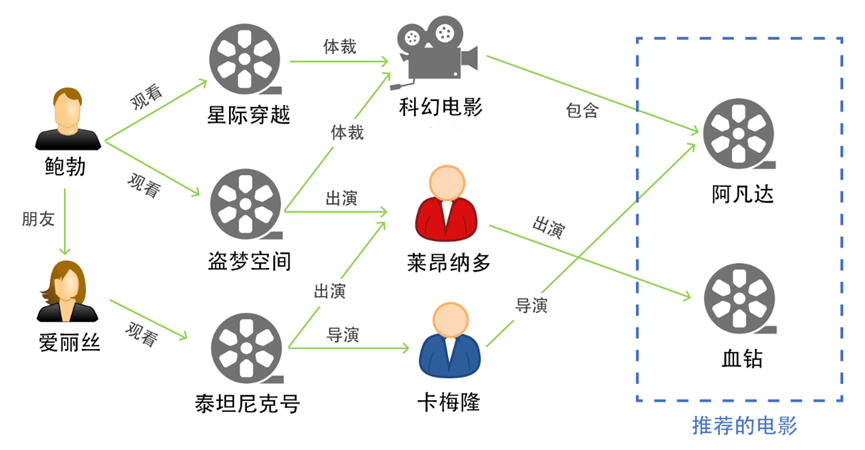
\includegraphics[width=\textwidth]{figures/enhanced-recommendation.png}
	\bicaption{基于知识图谱的电影推荐系统}{Knowledge graph enhanced movie recommendation system}\label{fig:enhanced-recommendation}
\end{figure}

(1)知识图谱引入了实体语义相关性,这可以帮助找到实体间潜在的联系并提高推荐物品的准确性。

(2)知识图谱由各种类型的关系构成,这对合理地扩展用户兴趣并增加推荐商品的多样性是有益的。

(3)知识图谱连接用户的历史记录及推荐的商品,因此提高了推荐系统的可解释性。

将知识图谱作为辅助信息加入至推荐系统中是当前的热点问题,目前基于知识图谱构建推荐系统的方法主要有以下几类:

(1)基于嵌入的方法。基于嵌入的方法通过知识图谱嵌入计算算法将知识图谱中的实体信息与关系信息映射为低维向量空间中的向量表示(嵌入表示)。而后推荐算法利用该嵌入表示来完成相应的计算,并给出推荐结果。目前将知识图谱中嵌入表示信息作为辅助信息的推荐模型有CKE\cite{zhang2016collaborative}、DKN\cite{wang2018dkn}以及SHINE\cite{wang2018shine}等。CKE是微软在 KDD2016 年发表的,其模型结构在原有系统过滤得到$U$, $V$向量的基础上,将物品的嵌入与其他描述信息相结合,这些信息主要有:
采用 TransR 算法嵌入得到的知识图谱,图谱内每个实体嵌入表示被提取为物品的结构化向量信息。
采用SDAE模型得到物品描述性文本的文本嵌入表示。
采用SCAE模型得到物品相关图像的视觉嵌入表示。DKN是之前同样由微软团队在WWW2018会议上发表的。它是一个主要针对新闻推荐任务提出的框架,知识图谱用于辅助计算新闻标题的嵌入表示。DKN提出对新闻标题内每一个关键实体,在知识图谱内找到其实体嵌入和上下文嵌入。
SHINE设计深度自编码器来嵌入语义网络,社交网络并进行推荐。其为用户-物品的交互使用自动编码器并计算用户感兴趣的概率。此外,嵌入表示可以包含实体的独热编码\cite{koren2008factorization}、词汇集\cite{wang2018dkn}、上下文信息\cite{sun2017collaborative}或属性\cite{wang2018shine},而选择哪一种嵌入向量的计算方式取决于其应用场合。

(2)基于路径的方法。基于路径的方法将知识图谱作为异构信息网络,主要是通过知识图谱中的路径关系信息来辅助推荐算法完成推荐相关的计算工作。目前基于知识图谱中路径信息的推荐模型有HIN\cite{zhao2017meta}、RKGE\cite{sun2018recurrent}等。HIN是2017年在KDD上提出的,与PER\cite{yu2014personalized}类似,都将知识图谱作为异构信息网络。它针对Yelp和Amazon数据集分别设计了元路径,并得到了L个评估函数。并在建模时使用FM模型,使用FM损失函数组进行梯度下降,并最终得到推荐结果。RKGE模型使用了基于循环神经网络的方法。在人为定义元路径并抽取出所有路径之后,对每种元路径都使用循环神经网络模型来抽取并推理其路径中所包含的信息。

(3)混合式方法。基于嵌入的方法未能充分利用实体间的关系模式信息,而基于路径的方法仅考虑了实体间的语义连通信息,未能有效使用用户/物品本身的语义信息。因此,目前出现了混合式方法,即同时结合了基于嵌入的方法与基于路径的方法的优点。混合式方法是当前的研究热点与焦点,使用该方法的典型模型有AKUPM\cite{tang2019akupm}和RCoLM\cite{cao2019unifying}等。AKUPM是通过注意力机制增强的推荐模型,RCoLM则是基于联合学习并以任务为导向的推荐算法。本文实现的电影推荐系统基于文献\parencite{wang2018ripplenet},其所使用的算法模型是也属于混合式方法。
\section{本文的主要研究内容}
本文在推荐算法、知识图谱和基于知识图谱的推荐算法的相关研究基础上,做了以下三方面的研究:

(1)对推荐系统所需的数据进行采集和处理,使用“MovieLens 1M Dataset”作为数据集,此外还从IMDb及豆瓣网爬取了相关电影数据并进行处理,作为本文的研究对象。

(2)根据文献\parencite{wang2018ripplenet}提出的算法,实现了基于知识图谱的涟漪网络推荐算法,此算法能根据用户的历史行为为用户进行电影推荐。不同于文献\parencite{wang2018ripplenet}中仅使用用户评分计算用户偏好,本文在用户偏好的计算过程中还结合了用户收藏,这在一定程度上缓解了冷启动问题并改进了推荐性能。此外,将涟漪网络算法与其他基于知识图谱的推荐算法(DKN\cite{wang2018dkn}、CKE\cite{zhang2016collaborative} 、PER\cite{yu2014personalized}、SHINE\cite{wang2018shine}、LibFM\cite{rendle2012factorization}和Wide\&Deep\cite{cheng2016wide}等)进行了性能比较。

(3)实现了一个基于知识图谱的电影推荐系统,该系统能够根据用户的历史行为(评分、收藏等)来为用户进行电影推荐。该系统分为管理员、未登录用户、普通登录用户。管理员能增加、修改和删除电影和普通用户;未登录用户能根据电影分类查看电影列表以及查看电影详情;普通登录用户除了能进行未登录用户的所有操作外,还能购买、收藏及为电影评分。
\section{论文结构}
本论文一共分为五个章节。

第1章是绪论。简明介绍知识图谱作为辅助信息在推荐算法中的作用以及推荐算法对在线流媒体播放平台的作用,同时介绍了推荐系统、知识图谱和基于知识图谱的推荐系统的发展和应用,并说明了本文的主要工作。

第2章是相关理论和技术。介绍了目前知识图谱和推荐系统的研究现状,并对传统的推荐算法与加入辅助信息的推荐算法作了较为细致的分类与阐述。同时还介绍了本文实现的电影推荐系统所使用的技术栈,诸如数据库、前端架构、后端架构等。

第3章是涟漪网络。介绍了涟漪网络算法,以及计算相关实体嵌入的过程中使用的深度学习算法,并对以上算法进行了讨论。最后,还对涟漪网络推荐算法的准确度进行了测试。

第4章是电影推荐系统。介绍了以涟漪网络算法为基础构建的电影推荐系统:介绍了系统架构、系统功能、电影推荐流程以及如何保证该系统的安全性。

第5章是研究结论和展望。总结了涟漪网络算法的设计与实现、电影推荐系统的功能,并指出了其中可以改进的地方。
\chapter{相关理论和技术}
\section{知识图谱}
\subsection{知识图谱的概念及发展进程}
知识图谱,是一种知识可视化或知识领域映射地图,是显示知识发展进程与结构关系的一系列三元组(实体,关系,实体),用可视化技术描述知识信息及其载体,挖掘、分析、建立、绘制和可视化知识以及实体之间的相互关系。

知识图谱是谷歌于2012年提出的,目的是为了增强其搜索引擎。而后微软于2013年7月发布了Microsoft Satori知识图谱。除传统搜索服务提供商之外,包括Apple,Facebook,IBM等互联网企业也在探索该领域。此外,业界也出现了社区构建的开源知识图谱,如DBpedia,NELL和Wikidata等。以Freebase、WordNet和GeneOntology等为例的知识图谱已成为支持人工智能相关应用的非常重要的资源。
\subsection{知识图谱的构建方法}
知识图谱是由多实体结点和不同关系边构成的多关系图,一个边是一个事实三元组(头结点,关系,尾结点),记为$(h,r,t)$。而知识图谱的构建便是寻找这样的三元组。

在过去十年间,出现了诸多构建大型知识图谱的方法,然而,还没有清晰准确的构建知识图谱的范式。主要有两个困难:(1)知识图谱是符号化的逻辑系统而知识图谱的应用常常包含在连续空间中的计算;(2)在一张知识图谱上进行知识聚合是困难的。

目前,知识图谱主要通过以下3个步骤来完成构建:

(1)信息抽取。即从各类型的源数据中抽取出实体(概念)、实体间的关系,并在此基础之上形成确切的知识表达。

(2)知识融合。对新获得的知识进行整合,以完成消歧义。

(3)知识加工。经过质量核查后将融合后的新知识的正确的部分加入至知识图谱中。
\subsection{知识图谱的应用}
知识图谱以更接近人类认知的方式为互联网的信息表达提供了一种新的方式,而且提供了一种更益于组织与利用海量数据的方式。当前知识图谱主要用于推荐系统、搜索引擎、个人助理以及问答系统。
\section{推荐系统}
推荐系统是内容过滤系统的一个子集,被广泛使用于多个领域,它向用户推荐满足其偏好的物品,并通常具有为视频或音乐服务生成推荐清单的表现形式。
\subsection{传统的推荐系统}
传统的推荐系统主要分为基于内容的推荐系统、基于协同过滤的推荐系统和混合推荐系统\cite{黄立威2018基于深度学习的推荐系统研究综述}。基于内容的推荐系统主要用于文本相关的项目,因为内容常常是使用关键字来描述的。该算法通过计算相关物品的离散特征,然后推荐具有与用户历史偏好物品类似特征的有关物品。基于协同过滤的推荐系统主要通过将具有与目标用户相似特征的用户所交互过的物品推荐给目标用户。

基于内容的推荐与基于协同过滤的推荐的有关区别可以通过比较两个流行音乐推荐系统的实现方式看出。(1)潘多拉音乐使用一个基于内容推荐的推荐算法。它根据艺人或歌曲的属性来生成一个包含相似风格歌曲的电台,并且该电台的内容会根据收听用户的反馈进行调整。当用户对一首歌曲“不感兴趣”时该算法将弱化该歌曲的一些属性;而当用户喜欢一首歌曲时,将强化一些属性。并且该算法会根据该属性调整歌曲的顺序,若属性的值越过一个阀值时推荐算法便将某一歌曲从列表中删除。(2)“终级fm”使用协同过滤的推荐算法。它记录用户经常收听的乐队和歌手,然后与其它用户的有关行为进行比较,建立一个电台,并以此推荐歌曲。“终级fm”会给用户推荐其他具有相似特征用户的播放列表(并保证目标用户未收听过)。

基于内容的推荐与基于协同过滤的推荐各有优缺点。潘多拉音乐所使用的基于内容推荐的推荐算法是根据物品本身的性质来进行推荐的,因此不需要用户信息就可以有较好的准确度。但该算法严重依赖物品本身的特性,因此局限性较大,推荐的内容都是与种子集相关的,推荐结果的多样性较低。而“终级fm”使用的协同过滤算法需要根据用户与物品的交互来生成推荐结果,因此需要大量的用户数据,存在数据稀缺性问题与冷启动问题。
\subsection{基于知识图谱的推荐系统}
基于内容推荐与协同过滤推荐两者均存在一些局限性,为了提高推荐的准确性,解决传统推荐算法的数据稀缺性与冷启动问题,研究者将一些辅助信息加入至推荐算法中,通常这些辅助信息包括上下文信息、用户或物品的属性、图片和社交网络\cite{常亮2019知识图谱的推荐系统综述, 秦川2020基于知识图谱的推荐系统研究综述}。

而随着知识图谱的发展,将知识图谱作为辅助信息来提高推荐系统的性能已经成为了热门的研究方向。将知识图谱作为辅助信息加入推荐算法的优点有:

(1)提高推荐系统的准确性。知识图谱可以表示不同实体间的关系,可以将物品及其相关属性对应于知识图谱之中,从而推荐算法可以理解物品之间的关系。此外,用户与用户间的关系信息也可以映射至知识图谱之中,从而推荐算法可以更准确地分析物品与物品间的关系、用户与物品之间的关系。
    
(2)提高推荐系统的可解释性。由于推荐结果依照知识图谱中的关系信息,因此可以由知识图谱中的关系路径得到推荐系统给出推荐结果的原因。

目前主要的基于知识图谱的推荐算法有基于嵌入的方法、基于路径的方法以及混合式方法:

(1)基于嵌入的方法。基于嵌入的方法使用知识图谱的信息来完善实体的嵌入表示。为了将知识图谱中的信息添加至推荐算法中来辅助推荐,需要使用知识图谱嵌入表示算法(Knowledge Graph Embedding, KGE)表计算实体嵌入(实体嵌入指由知识图谱中的信息得到的在低维向量空间中的向量表示)。KGE算法有TransE\cite{bordes2013translating}、TransH\cite{wang2014knowledge}、TransR\cite{lin2017learning}和DistMult\cite{yang2014embedding}等。而推荐算法利用该嵌入表示来进行相关计算,从而对用户进行物品推荐。

(2)基于路径的方法\cite{lin2015modeling, guu2015traversing, toutanova2016compositional}。基于路径的方法将知识图谱视为异构信息网络。而推荐系统利用该异构信息网络寻找实体间的关系,从而完成推荐。

(3)混合式方法。基于嵌入的方法未能充分利用实体间的关系模式信息,而基于路径的方法仅考虑了实体间的语义连通信息,未能有效利用用户/物品本身的语义信息。混合式方法结合了基于嵌入的方法与基于路径的方法的优点,该方法是当前的研究热点与焦点,使用该方法的典型模型有AKUPM\cite{tang2019akupm}和RCoLM\cite{cao2019unifying}等。本文实现的算法属于混合方法。
\section{系统开发技术}
\label{sec:tech-stack}
\subsection{数据采集技术}
电影推荐系统使用的数据来自“MovieLens 1M Dataset”\footnote{https://grouplens.org/datasets/movielens/1m/}数据集,此外还从IMDb\footnote{https://www.imdb.com/}及豆瓣网\footnote{https://www.douban.com/}爬取了相关电影数据并进行处理作为本文的研究对象。

在数据采集的过程中,使用Scrapy框架进行了数据爬取,爬取的数据包括电影名称、电影封面、预告片图片、电景情节介绍、导演、演员以及剧作家。

最终,总计爬取了3684部电影的数据。其中,从IMDb爬取了3494条电影数据,从豆瓣爬取了190条电影数据(由于豆瓣网限制了每IP访问量故爬取的数据较少)。
\subsection{数据存储技术}
本系统使用MongoDB与Neo4j存储数据。

\noindent (1)MongoDB

MongoDB是一个新兴的非关系型存储的分布式存储数据的数据库,属于NoSQL,与MySQL等传统的关系型数据库相比,它提供更好的高并发支持,具有高可靠性的优点。与此同时,得益于其基于文档储存的特点,相比较传统的关系型数据库,它的存储结构更灵活。

在本系统中,MongoDB存储普通用户数据、管理员数据、电影数据等。

\noindent(2)Neo4j

Neo4j是一个具有高性能的图数据库,它将结构化的数据信息储存在网络上而不是存储在表中。它具有健壮和成熟的数据库的所有特点。虽然Neo4j是一个新兴的数据库,但它已在具有超过1亿节点、关系和属性的产品中得到了应用,充分体现了其高性能、高可靠性的特点。

在本系统中,最终需存储的图结点有182011个,需存储的边有1241995条。如果将它们存储在传统的关系型数据库中,会因大量的连接查询导致极大的性能开销,表现为查询耗时久。Neo4j对图数据处理做了优化,因此查询等操作可以在较短的时间内完成,故本系统将知识图谱数据存储在Neo4j中而不是关系型数据库中。

\subsection{后端技术}
本系统使用Flask框架作为网站后端框架。Flask是一个Python编写的轻量级微框架。它具有轻量、便捷、可扩展等特点。系统使用Flask框架充分利用了其便捷、可扩展以及开发便捷的特点,与本系统要求相符。

系统使用表现层状态转换(REST)风格的应用程序接口(API)作为前后端的交互接口。表现层状态转换(Representational State Transfer,REST)是一种基于HTTP协议的软件交互体系结构样式,该协议是由Roy Thomas Fielding博士在2000年的博士论文中引用的\cite{fielding2000architectural},目的是促进不同的软件/程序的开发。在网络上互相传输数据。表示层状态转换基于超文本传输​​协议(HTTP)的一组约束,该协议是一种旨在提供万维网服务的软件构造样式。符合或兼容此体系结构样式(简称为REST或RESTful)的网络服务允许客户端发出使用统一资源标识符访问和操作网络资源的请求,这些资源与一组预定义的操作一致。因此,表示层状态转换提供了Internet上计算机系统之间相互使用资源的互操作性。与其他类型的网络服务(例如SOAP服务)相比,它们使用自己定义的一组操作来访问网络资源。

得益于本系统使用了REST风格的API,本系统能更有效地使用缓存来提升响应速度,同时前后端间的通讯的无状态性可以让不同的服务器处理一连串请求中不同的请求,提高了本系统的可扩展性。与此同时,得益于REST风格语义化的接口,使前后端交互接口更清晰明了,使接口的使用者能更高效便捷地进行相关的开发工作。
\subsection{前端技术}
本系统前端使用Angular框架。Angular(通常指“Angular 2+”或“Angular v2及以上”)是一个基于TypeScript的开源网络应用框架,它的开发由Google的Angular团队领导同时也有个人及其他公司维护。Angular完全从相同团队开发的AngularJS重新编写而来。Angular常常作为MEAN技术栈的一部分。MEAN技术栈指MongoDB数据库、Express.js网络服务器框架、Angular/AngularJS以及Node.js服务器运行时。不同于MEAN技术栈,本系统将其中的“E”(指Express.js网络服务器框架)替换为了Flask网络服务器框架。

通过使用Angular框架,本系统具有一个现代化、模块化、响应式的网页架构。同时借助于Angular Material Components官方组件库,本系统前端UI符合材料设计(Material Design)。
\chapter{基于涟漪网络知识图谱的推荐算法}
\label{ch:offline-recommendation}
\section{涟漪网络}
本算法基于文献\parencite{wang2018ripplenet}实现,并在其基础上进行了一定的改进:文献\parencite{wang2018ripplenet}中计算用户偏好时并未考虑用户收藏,本文在计算用户偏好时,将用户收藏考虑在内,这在一定程度上缓解了数据稀缺性问题和冷启动问题并改进了推荐性能。
\subsection{架构}
涟漪网络的总体架构如图\ref{fig:ripplenet-framework}所示,图上方的知识图谱中展示了由用户交互产生的涟漪。涟漪网络以一个用户$u$和一个电影$v$作为输入,并输出用户$u$与电影$v$之间产生交互的概率。对输入用户$u$而言,其历史交互记录$V_u$是知识图谱中的种子集,而后沿着知识图谱中的关系边形成多个涟漪集$S_u^{k}\ (k=1, 2, \dots, H)$。第$k$个涟漪集是种子集$V_u$经过$k$跳得到的知识三元组。然后迭代地利用这些涟漪集与电影$v$的嵌入表示(黄色的块)计算出用户$u$对电影$v$的的响应(绿色的块),最后结合得到用户的最终嵌入表示(灰色的块)。最终,利用用户$u$与电影$v$的嵌入表示计算出用户$u$对电影$v$感兴趣的预测概率$y_{uv}$。
\begin{figure}
	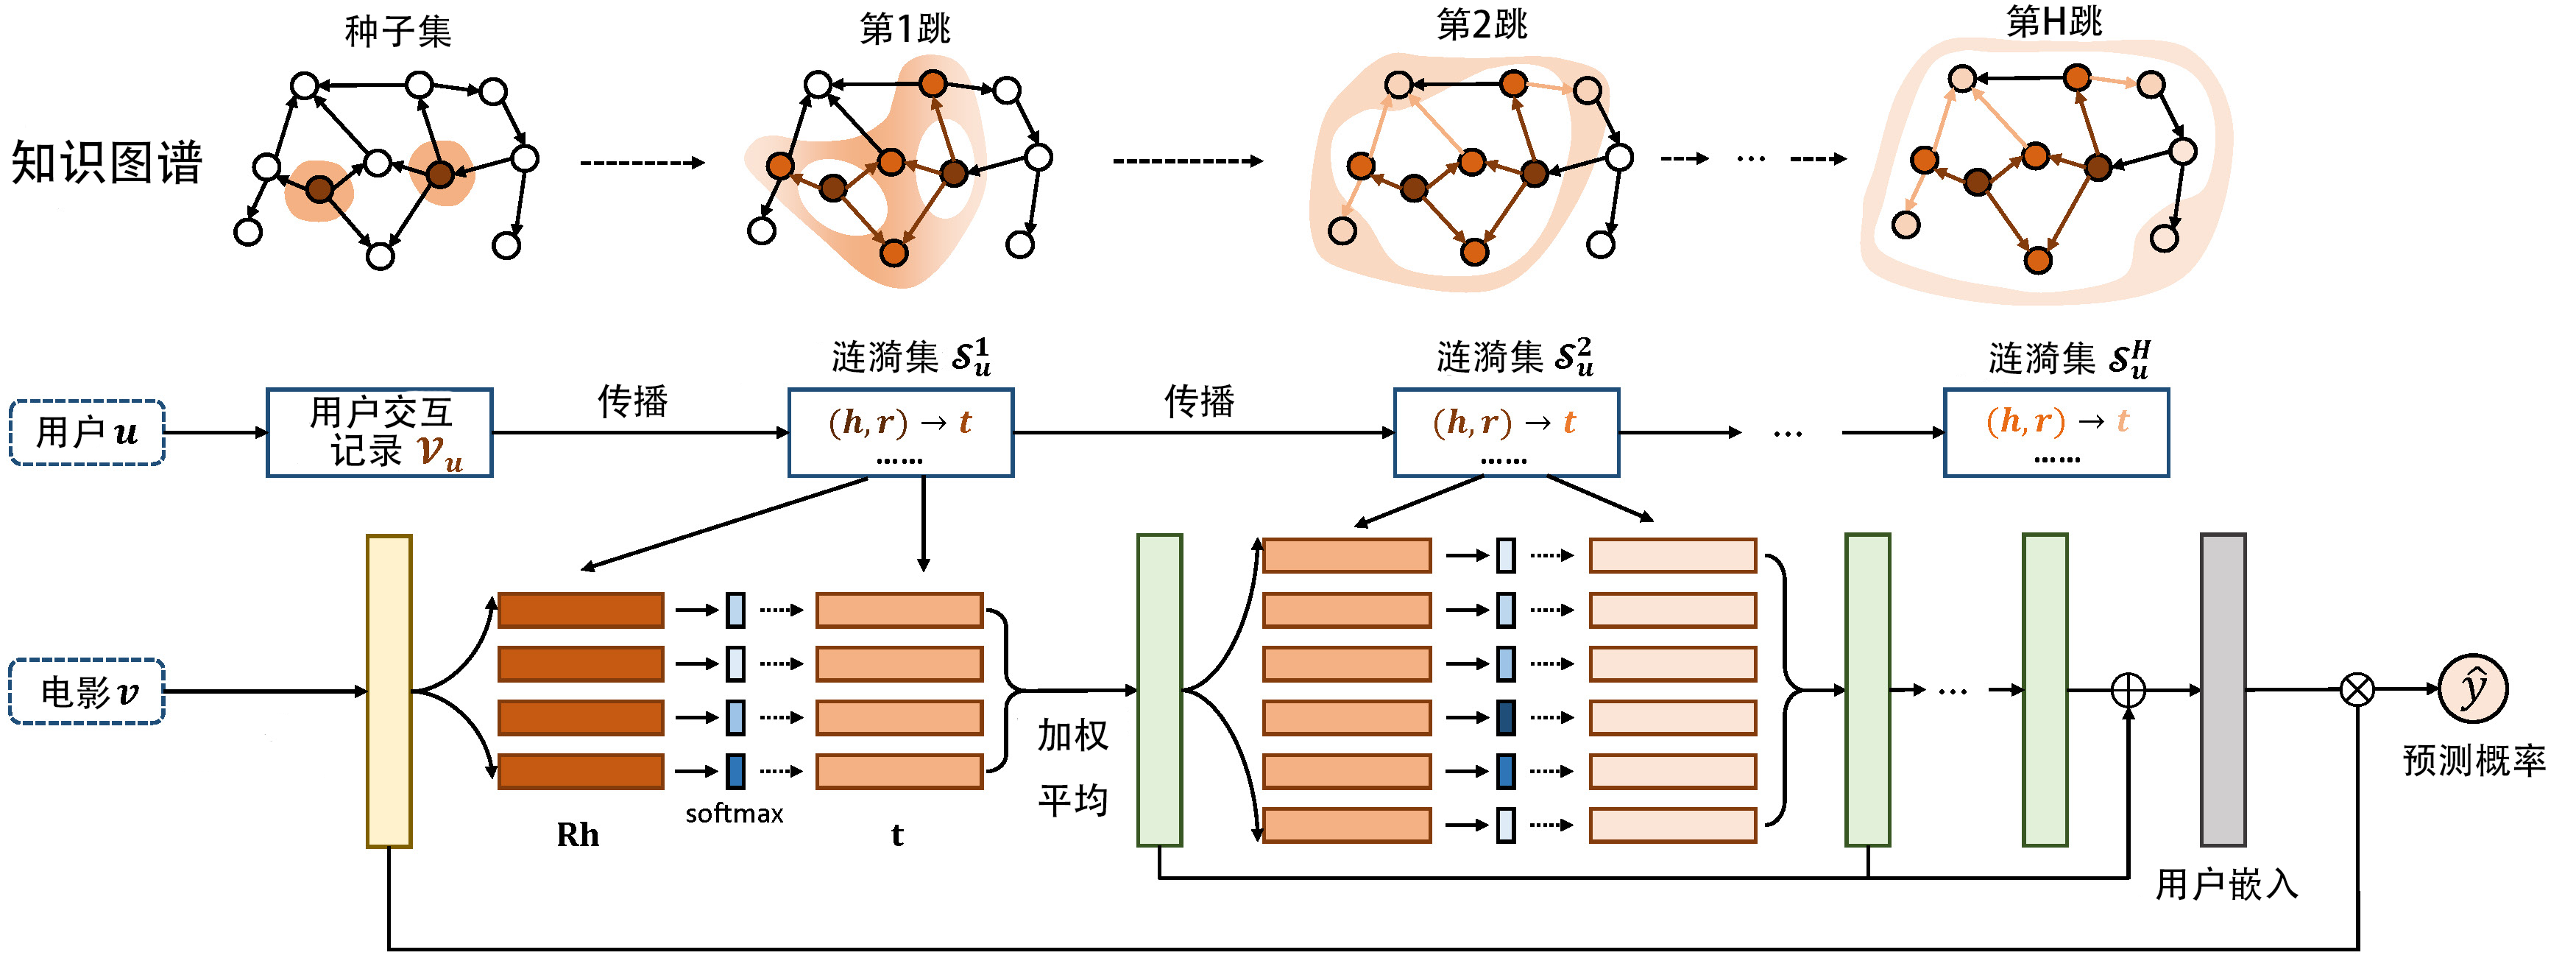
\includegraphics[width=\textwidth]{figures/ripplenet-framework.png}
	\bicaption{涟漪网络的总体架构}{The overall framework of the Ripple Network}\label{fig:ripplenet-framework}
\end{figure}
\subsection{涟漪集}
\begin{figure}
	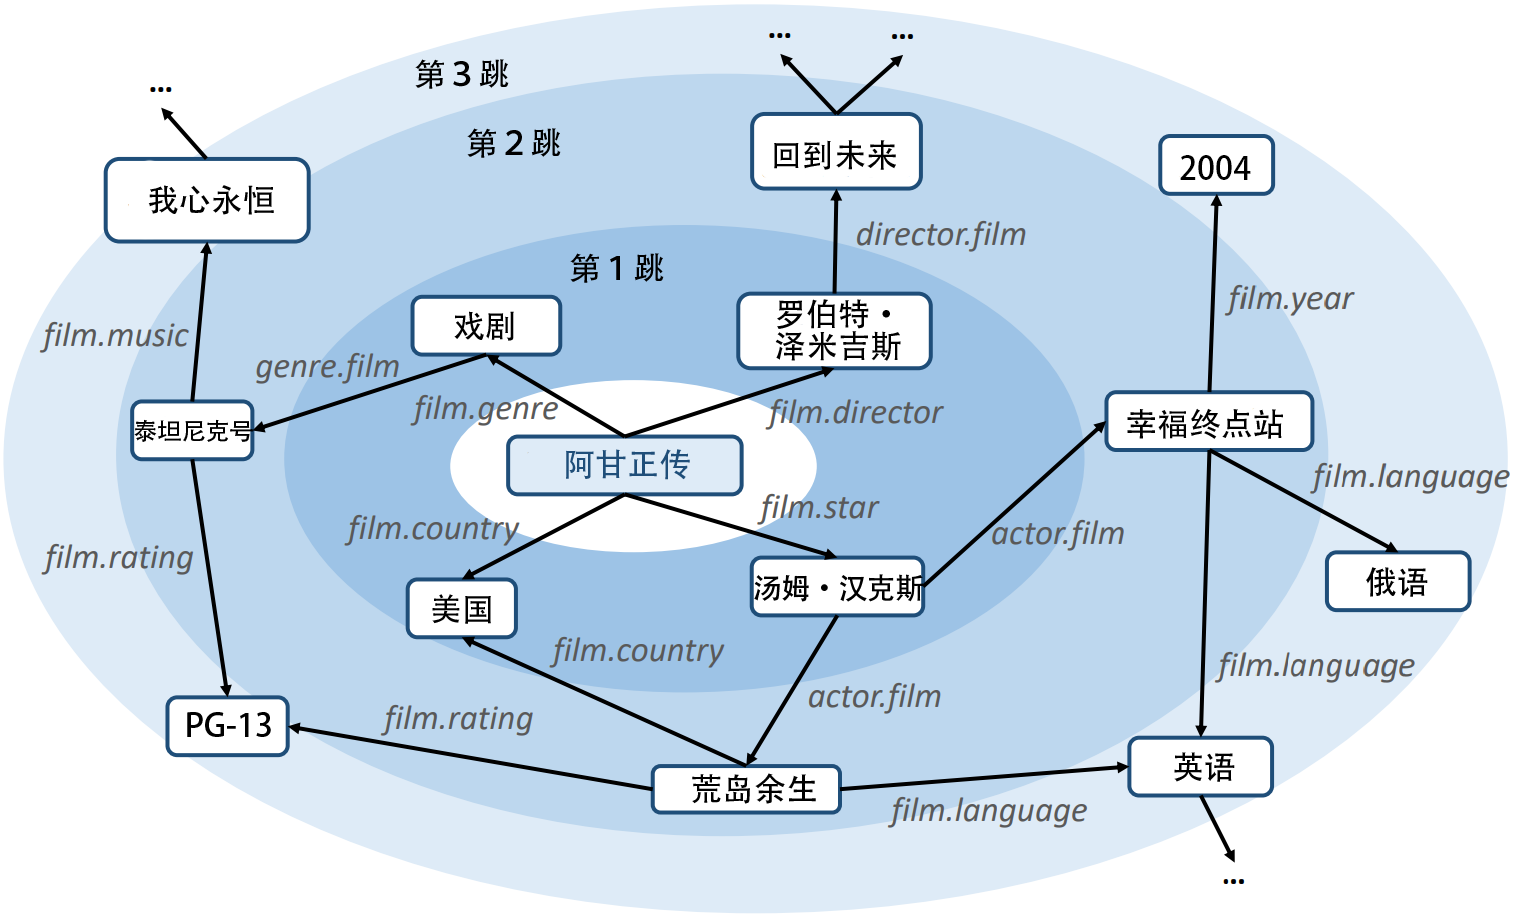
\includegraphics[width=\textwidth]{figures/illustration-of-ripple-sets.png}
	\bicaption{电影知识图谱中由“阿甘正传”激发的涟漪集}{Sets of ripples of “Forest Gump” in Knowledge Graph of movies}\label{fig:illustration-of-ripple-sets}
\end{figure}
知识图谱常常含有丰富的事实信息与实体间的联系。比如,图\ref{fig:illustration-of-ripple-sets}(图中不同颜色的圆圈表示不同跳数的涟漪集,越浅的蓝色代表种子集与该区域内实体的关联程度越低)中电影“阿甘正传”与“罗伯特·泽米吉斯”相连,它们之间的联系为“罗伯特·泽米吉斯”是电影“阿甘正传”的导演。而“回到未来”也与“罗伯特·泽米吉斯”相连。因此,如果一个用户与电影“阿甘正传”交互过,则他很有可能也对“回到未来”感兴趣。为了描述用户在知识图谱中分层次的潜在偏好集,递归定义用户$u$的$k$跳相关实体如下:

\textbf{定义1(相关实体集)} 给定交互矩阵$\Upsilon$与知识图谱$G$,则用户$u$的$k$跳相关实体集的定义为式\eqref{eq:relevant-entities}。

\begin{equation}
	E_u^k=\{t|(h, r, t)\in G \text{且} h\in E^{k-1}_u\}, k = 1, 2, \dots, H\label{eq:relevant-entities}
\end{equation}

式\eqref{eq:relevant-entities}中,$E_u^0=V_u=\{v | y_{uv}=1\}$是用户的历史偏好集(历史偏好集是指用户在最高为5的评分中给出的评分$\geqslant$4的物品以及用户已加入收藏的物品),可以看作是用户$u$在知识图谱中的种子集。

相关实体集可以看作是用户的历史偏好集在知识图谱中的自然扩展。给定相关实体集的定义,以下定义用户$u$的$k$跳涟漪集:

\textbf{定义2(涟漪集)}用户$u$的$k$跳涟漪集可以看作是知识图谱中以$E^{k-1}_u$为起点的知识三元组,定义如式\eqref{eq:ripple-set}所示。

\begin{equation}
	S_u^k = \{(h, r, t)|(h, r, t)\in G \text{且} h\in E^{k-1}_u\}, k = 1, 2, \dots, H\label{eq:ripple-set}
\end{equation}

“涟漪”这个词有两重意思:(1)对由多个雨点产生的真实涟漪的模拟,用户对电影的潜在兴趣集在知识图谱中由近及远地传递。这一过程如图\ref{fig:illustration-of-ripple-sets}所示。(2)用户的潜在兴趣随着知识图谱中传递的跳数$k$的增大逐渐递减。图\ref{fig:illustration-of-ripple-sets}中蓝色的变浅显示了潜在兴趣递减的过程。

一个可能出现的问题是在跳数$k$增加的过程中涟漪集的大小可能过大。为了解决这个问题,注意到:

(1)在真实使用的知识图谱中大量的实体是沉没实体,意思是它们只有传入链路而没有传出链路。

(2)在电影推荐的具体情境下,关系可以限制在情境相关的分类中以减少涟漪集的数量并提高实体间的相关度。

(3)最大跳数$H$通常在实际应用中不会过大,因为离用户历史偏好集较远的实体会带来更多的错误推荐而不是更丰富的推荐结果。

(4)在涟漪网络中,我们可以对一个固定大小的邻集而不是对完整的涟漪集采样从而更进一步地减小计算工作量。设计这样的采样器是一个重要的工作,尤其是非统一的采样器能更好地捕获用户的分等级的潜在兴趣。
\subsection{偏好扩散}
\label{sec:osum}
传统的协同过滤算法是通过学习用户与物品间的潜在联系来完成推荐,而在涟漪网络算法中,这一过程是通过偏好扩散完成的:对每个用户,涟漪网络将他的过往兴趣视为知识图谱中的种子集,然后沿知识图谱中的路径不断地拓展用户的潜在兴趣集,进而得到按等级划分的关于候选物品的潜在兴趣集。我们利用现实生活中的由雨滴产生的涟漪在水面上扩散来模拟偏好扩散的过程,其中多个“涟漪”重叠形成基于知识图谱的用户偏好分布。

如图\ref{fig:ripplenet-framework},每部电影都有一个嵌入表示$v$,$v\in \mathbb{R}^{d}$,其中$\mathbb{R}$是实数集,$d$是嵌入表示向量的维数。给定电影的嵌入表示$v$以及用户$1$跳涟漪集$S_u^{1}$,可以利用电影$v$、$S_u^{1}$中的三元组中头节点$head_i$以及该三元组中的关系$r_i$来计算出电影$v$和实体$head_i$之间的相关度,如式\eqref{eq:item-entity-relevance}所示。

\begin{equation}
	p_i=softmax(v^TR_ih_i)=\frac{exp(v^TR_ih_i)}{\sum_{(h, r, t)\in S_u^1} exp(v^TRh)}\label{eq:item-entity-relevance}
\end{equation}

式\eqref{eq:item-entity-relevance}中,$R_i\in \mathbb{R}^{d\times d}$与$h_i\in \mathbb{R}^d$分别是关系$r_i$和头节点$h_i$的嵌入表示。相关度$p_i$为向量空间$R_i$中的电影$v$与实体$h_i$之间的相似度。同时还考虑了关系信息的嵌入表示矩阵在计算电影$v$与实体$h_i$之间的相似度,因为不同电影-实体对之间的相似度在不同关系的场景下可能有所不同。比如,“阿甘正传”与“回到未来”在导演方面有很高的相似度,但它们在体裁或剧作家方面可能没有联系。

在完成相似度计算之后,将$S_u^{1}$中三元组的尾节点根据计算得到的相似度进行加权求和,得到向量$o^{1}_u$,如式\eqref{eq:o1}所示。

\begin{equation}
	o^1_u=\sum_{(h_i,r_i,t_i)\in S_u^1}p_it_i\label{eq:o1}
\end{equation}

式\eqref{eq:o1}中,$t_i\in \mathbb{R}^{d}$,$t_i$是事实三元组中的尾节点。向量$o^{1}_u$可以视为用户偏好集$V_u$关于电影$v$的$1$次响应。与协同过滤算法类似的是,它根据用户交互过的物品来表示用户嵌入而不是使用单独的参数来表示用户,从而减少了参数数量。通过式\eqref{eq:item-entity-relevance}与式\eqref{eq:o1},用户的偏好从其交互过的电影(即种子集)成功在知识图谱中进行了一次扩散,这称为涟漪网络中的偏好扩散。

可以将式\eqref{eq:item-entity-relevance}中的$v$替换为$o_u^1$,我们可以再次进行偏好扩散以得到用户的2次响应$o_u^2$。以此类推,最终我们可以将该用户的偏好集扩散至$H$跳,得到用户的涟漪集$S_u^{i}, i=1,\dots,H$。从中可以得到用户的多次响应$o^{1}_u, o^{2}_u, o^{H}_u$。用户$u$关于电影$v$的嵌入表示是通过结合所有的不同响应并计算得到的,如式\eqref{eq:osum}所示。
\begin{equation}
	u=o_u^1+o_u^2+\dots+o_u^H\label{eq:osum}
\end{equation}

尽管最后一跳的用户响应中理论上包含了所有之前得到的信息,但是对$o^k_u$进行求和仍然是有必要的,因为之前得到的用户响应可能在偏好传递的过程中稀释了,因此仅使用最后一跳的响应不能很好地表示用户嵌入。最终,利用用户嵌入与电影嵌入,计算出用户对电影感兴趣的概率,如式\eqref{eq:predicted-possibility}所示。
\begin{equation}
	y_{uv}=\zeta(u^Tv)\label{eq:predicted-possibility}
\end{equation}

其中,$\zeta(x)=\frac{1}{1+exp(-x)}$是sigmoid函数。
\section{学习算法}
在涟漪网络算法中,我们的目标是通过式\eqref{eq:predicted-possibility}求出用户对电影感兴趣的概率。但是,为了将其计算出来我们需要先求出所有物品、用户以及关系的嵌入表示,如第\ref{sec:osum}节中所述,用户的嵌入表示可以通过其涟漪集来代替,以此消元。但物品及关系的嵌入表示却是需要求出来的。

为了求出物品及关系的嵌入表示,这里使用最大后验概率估计的方法。

我们的目标是在已经得到知识图谱$G$以及用户与电影的交互矩阵$\Upsilon$的情况下最大化模型参数$\Gamma$,如式\eqref{eq:max}所示。
\begin{equation}
	max\ p(\Gamma |G,\Upsilon)\label{eq:max}
\end{equation}

式\eqref{eq:max}中,参数$\Gamma$包含了全部的实体、关系和电影的嵌入表示。可以将式\eqref{eq:max}等价于最大化式\eqref{eq:equal-max}。

\begin{equation}
	p(\Gamma |G,\Upsilon)=\frac{p(\Gamma,G,\Upsilon)}{p(G,\Upsilon)}\varpropto p(\Gamma)\centerdot p(G|\Gamma)\centerdot p(\Upsilon|\Gamma,G)\label{eq:equal-max}
\end{equation}

根据贝叶斯公式,在式\eqref{eq:equal-max}中,第一项$p(\Gamma)$代表模型参数的先验概率。设$p(\Gamma)$为均值为0,方差为对角协方差矩阵的正态分布,如式\eqref{eq:normal-distribution}所示。

\begin{equation}
	p(\Gamma)=N(0,\lambda_1^{-1}I)\label{eq:normal-distribution}
\end{equation}

式\eqref{eq:equal-max}中,$p(G|\Gamma)$是给定$\Gamma$的知识图谱的最大似然函数。最近,有研究者提出了多种计算知识图谱嵌入的方法,包括基于距离的方法和基于语义匹配的方法。在本算法中,使用三路张量分解的方法来建立知识图谱嵌入的最大似然函数,如式\eqref{eq:term2}。

\begin{equation}
	p(G|\Gamma)=\prod_{(h,r,t)\in E\times R\times E}p((h,r,t)|\Gamma)=\prod_{(h,r,t)\in E\times R\times E}N(I_{h,r,t}-h^TRt,\lambda_2^{-1})\label{eq:term2}
\end{equation}

式\eqref{eq:term2}中,若$I_{h,r,t}\in G$则标志$I_{h,r,t}$等于1,否则为0。式\eqref{eq:equal-max}中的第三项是给定$\Gamma$与知识图谱的似然函数,可以看作伯努利分布的累乘,如式\eqref{eq:bernoulli}。

\begin{equation}
	p(\Upsilon|\Gamma,G)=\prod_{(u,v)\in \Upsilon}\zeta(u^Tv)^{y_{uv}}\centerdot (1-\zeta (u^Tv))^{1-y_{uv}}\label{eq:bernoulli}
\end{equation}

对式\eqref{eq:equal-max}取负对数,有如式\eqref{eq:term3}所示的损失函数:
\begin{multline}
	min\ L=-log(p(\Upsilon|\Gamma,G)\centerdot p(G|\Gamma)\centerdot p(\Gamma))\\
=\sum_{(u,v)\in \Upsilon}-(y_{uv}log\ \zeta(u^Tv)+(1-y_{uv}log(1-\zeta(u^Tv))))\\
+\frac{\lambda_2}{2}\sum_{r\in R}\|I_r-E^TRE\|_2^2+\frac{\lambda_1}{2}(\|V\|^2_2+\|E\|^2_2+\sum_{r\in R}\|R\|^2_2)\label{eq:term3}
\end{multline}

式\eqref{eq:term3}中,$V$和$E$是所有电影与实体的嵌入表示,$I_r$是在知识图谱中对关系$r$的标志向量$I$的分向量。在式\eqref{eq:term3}中,第一项是交互矩阵$\Upsilon$与涟漪网络的估测值之间的交叉熵,第二项是真实的知识图谱分向量$I_r$以及人为构建的指示矩阵$E^{T}RE$之间的均方误差,最后一项是为防止过拟合加入的正则项。

直接求解上式来得到参数$\Gamma$是不可能的,因此可以使用随机梯度下降算法递归地优化损失函数来求解模型参数,而后再计算参数$\Gamma$的损失函数的梯度,并根据采样得到的一小批数据反向传递,然后更新参数并最终得到参数$\Gamma$。
\section{分析}
\subsection{可解释性}
可解释的推荐系统旨在阐释为什么用户会对一件物品感兴趣,这帮助提升用户对推荐结果的满意度以及对推荐系统的信任。对推荐结果的解释通常基于标签、语义分析等。因为涟漪网络探索用户基于知识图谱的兴趣,因此它提供了一种基于知识图谱中的关系路径来阐述推荐结果的全新方式。比如,在图\ref{fig:illustration-of-ripple-sets}中,当用户对“幸福终点站”感兴趣,则该用户也可能对“荒岛余生”感兴趣。因为在知识图谱中,“汤姆·汉克斯”与“幸福终点站”相连,关系是演员,而“汤姆·汉克斯”与“荒岛余生”也相连,关系也是演员,换句话说,“荒岛余生”与“幸福终点站”有相同的演员。这便解释了用户对“幸福终点站”和“荒岛余生”同时感兴趣的原因。涟漪网络算法通过在知识图谱中寻找与用户交互过的电影(种子集)相连的物品,并不断扩散,最终确保推荐结果具有较高的准确性。
\subsection{涟漪重叠}
在涟漪网络中,一个可能的问题是涟漪集中的电影非常多,从而在偏好传递的过程中不可避免地导致用户的真实潜在偏好信息被稀释。然而,用户点击记录中不同的电影常常高度重叠(从种子集出发到达一部电影常常有不止一条路径),这在很大程度上避免了真实潜在偏好信息被稀释的问题。比如,在图\ref{fig:illustration-of-ripple-sets}中,如果一个用户喜欢“阿甘正传”,则他也可能喜欢“荒岛余生”。在该知识图谱中,从“阿甘正传”到“荒岛余生”有两条路径:“阿甘正传-U.S.-荒岛余生”与“阿甘正传-汤姆·汉克斯-荒岛余生”,这正是涟漪重叠的表现。
\section{测试}
\subsection{数据集}
本测试使用“MovieLens 1M Dataset”数据集。该数据集由电影信息、用户信息以及用户对电影的评价三部分组成。其中,含有电影数据3883条、用户数据6040条以及1000209条用户对电影的评价数据。因该数据集数据量适中,数据准确可靠,因此在推荐系统的性能测试中被广泛使用。

本测试使用的知识图谱来自Microsoft Satori,是依据“MovieLens 1M Dataset”中的电影名称从Microsoft Satori中提取相关的节点的与关系数据得到的。
\subsection{基线}
本测试中,会将本算法的测试结果与以下算法的相比较:

DKN\cite{wang2018dkn}是由微软团队在WWW2018会议上发表的。它是一个主要针对新闻任务提出的框架,知识图谱用于辅助计算新闻标题的嵌入表示。DKN提出对新闻标题内每一个关键实体,在知识图谱内找到其实体嵌入和上下文嵌入。

CKE\cite{zhang2016collaborative}是微软在KDD2016年发表的,其模型结构在原有系统过滤得到$U$,$V$向量的基础上,将物品的嵌入与其他描述信息相结合,这些信息主要有:
采用TransR算法计算知识图谱嵌入表示,知识图谱内每个实体嵌入表示被提取为物品的结构化向量信息。
采用SDAE模型得到物品描述性文本的文本性嵌入表示。
采用SCAE模型得到物品相关图像的视觉嵌入表示。

SHINE\cite{wang2018shine}设计深度自编码器并嵌入语义网络以及社交网络来进行推荐。其为用户-物品的交互使用自动编码器并刻画用户感兴趣的概率。

PER\cite{yu2014personalized}是以基于路径的方法来将知识图谱作为辅助信息中的比较经典的算法。其提出的元路径可以为推荐系统提供可靠的方向,但是需要使用者了解领域内知识,进行人为路径设计。

LibFM\cite{rendle2012factorization}是一个广泛使用的在CTR场景中的分解推荐模型。

Wide\&Deep\cite{cheng2016wide}是一个结合线性路径的推荐模型。类似于LibFM,我们将用户、物品及实体的嵌入表示作为其输入。
\subsection{测试步骤}
在涟漪网络中,设置跳数$H=2$。根据实验结果,较大的跳数几乎无法提高性能却会造成较大的计算开销。我们将数据划分为训练集、评估集与测试集,按照6:2:2的比例进行分配。实验进行5次,计算准确度以及AUC然后取平均值。
\subsection{结果}
测试结果如表\ref{tab:acc-auc}中所示,总体上涟漪网络算法的性能最佳,其次是Wide\&Deep算法,说明他们可以充分利用知识图谱中的有效信息来辅助推荐算法。而表现最差的是PER算法,这可能是因为手工定义的元路径在电影推荐方面效果较差。
\begin{table}
	\bicaption{在兴趣预测计算中的AUC和准确度}{AUC and ACC in interest prediction}\label{tab:acc-auc}
	\begin{tabular}{ccc}
	 \toprule
	 算法 & AUC & 准确度 \\
	 \midrule
	 涟漪网络 & 0.899 & 0.835 \\
	  DKN & 0.655 & 0.589 \\
	  CKE & 0.796 & 0.739 \\
	  SHINE & 0.778 & 0.732\\
	  LibFM & 0.892 & 0.812\\
	  Wide\&Deep & 0.903 & 0.822\\
	  \bottomrule
	\end{tabular}
\end{table}
\chapter{基于知识图谱的电影推荐系统}
\section{系统整体设计}
如第\ref{sec:tech-stack}节中所述,本系统使用的数据来自“MovieLens 1M Dataset”、IMDb和豆瓣网。其中IMDb和豆瓣网的数据是使用爬虫爬取得到的。最后再使用Python脚本对这些数据进行处理加工,并导入MongoDB数据库和Neo4j数据库。

本系统使用MongoDB和Neo4j存储数据。其中,MongoDB作为非关系型的新兴NoSQL数据库,以灵活的非结构化的方式存储普通用户数据、管理员数据、电影数据等,并提供高并发的性能支持与可分布式存储的扩展性。而在以高性能著称的图数据库Neo4j中,存储用于推荐算法使用的电影知识图谱。

本系统后端使用Python编写的Flask框架,Flask框架是轻量级的微框架,以高可扩展性著称,为本系统的后端网页应用服务器提供支持。在Flask中,基于REST风格构建API以供前端使用,REST风格的语义化API使后端API的构建与前端API的使用简单方便。

本系统前端使用Angular作为前端网页框架。Angular是基于TypeScript的网页框架,以模块化及可重用的组件设计著称。Angular为本系统提供了模块化的网页设计,使本系统前端逻辑清晰,易于维护。此外,本系统使用了Angular材料组件库(Angular Material Components),得益于此,本系统遵循材料设计(Material Design)语言,使视觉传达风格简洁美观,具有响应式动化与过渡效过、光线与阴影等。
\section{数据库设计}
如前所述,本系统的MongoDB数据库用于存储普通用户数据、管理员数据、电影数据等,而Neo4j作为高性能的图数据库,用于存储知识图谱。以下逐一说明MongoDB数据库与Neo4j数据库的存储结构。

不同于MySQL等关系型数据库,MongoDB数据库作为非结构化存储的NoSQL数据库,没有表、列与行的概念,而只有集合与文档的概念,即在数据库中存储集合(一定程度上对应于关系型数据库的表),在集合中存储文档(一定程度上对应于关系型数据库的行),而关系型数据库中的列则对应于MongoDB数据库中文档的属性。

本系统在MongoDB数据库中建立4个集合,分别用于存储用户、管理员、体裁与电影数据。因其中的数据为非结构化数据,因此无法用表格的形式给出,目前习惯上以JSON形式给出数据的逻辑结构,以下以JSON形式来表示存储结构:

以下为普通用户集合的数据结构,用户集合中的文档存储用户ID、哈希处理后的密码、其进行过评分的电影(包括电影ID、评分及时间)以及由推荐算法服务器写入的推荐列表、已购买电影及心愿单:
\begin{verbatim}
    {
        _id: Integer,
        password: String,
        rating: Array([
            {
                movieId: Integer,
                rating: Integer,
                timestamp: Integer
            },
            ...
        ]),
        recommendation: Array([Interger, ...]),
        bought: Array([Interger, ...]),
        wishlist: Array([Interger, ...])
    }
\end{verbatim}

以下为管理员集合的数据结构,其存储结构较简单,管理员集合中的文档存储管理员ID、哈希处理后的密码:
\begin{verbatim}
    {
        _id: String,
        password: String
    }
\end{verbatim}

以下为体裁集合的数据结构,其存储结构较简单,体裁集合中的文档存储体裁名称:
\begin{verbatim}
    {
        _id: String
    }
\end{verbatim}

以下为电影集合的数据结构,电影集合中的文档存储电影ID、电影封面、体裁、价格、评分累加和、评分总数量、预告片图片、剧情介绍、导演、剧本作家及演员。需要说明的是评分累加和以及评分总数量对应于用户集合中的评分,但只起缓存作用,定期计算。(经测试表明,每次用户访问时计算的开销较大,用户得到响应的时间过长):
\begin{verbatim}
    {
        _id: Integer,
        title: String,
        cover: String,
        genres: Array([String, ...]),
        price: Float,
        ratingSum: Integer,
        ratingCount: Integer,
        trailer_image_url: String,
        storyline: Array([String, ...]),
        directors: Array([String, ...]),
        writers: Array([String, ...]),
        actors: Array([String, ...]),
    }
\end{verbatim}

Neo4j数据库用于存储推荐算法使用的知识图谱,含有182011个结点、1241995条边,其数据结构可表示为:
\begin{verbatim}
    node: actor | country | director | film | genre | language
        | person_or_entity_appearing_in_film | rating | star
        | writer
    relationship: actor.film | director.film | film.country
        | film.director | film.genre | film.language | film.rating
        | film.star | film.writer | genre.film
        | person_or_entity_appearing_in_film.film | writer.film
    edge = (node) - [relationship] -> (node)
\end{verbatim}
\section{系统功能说明}
\begin{figure}
	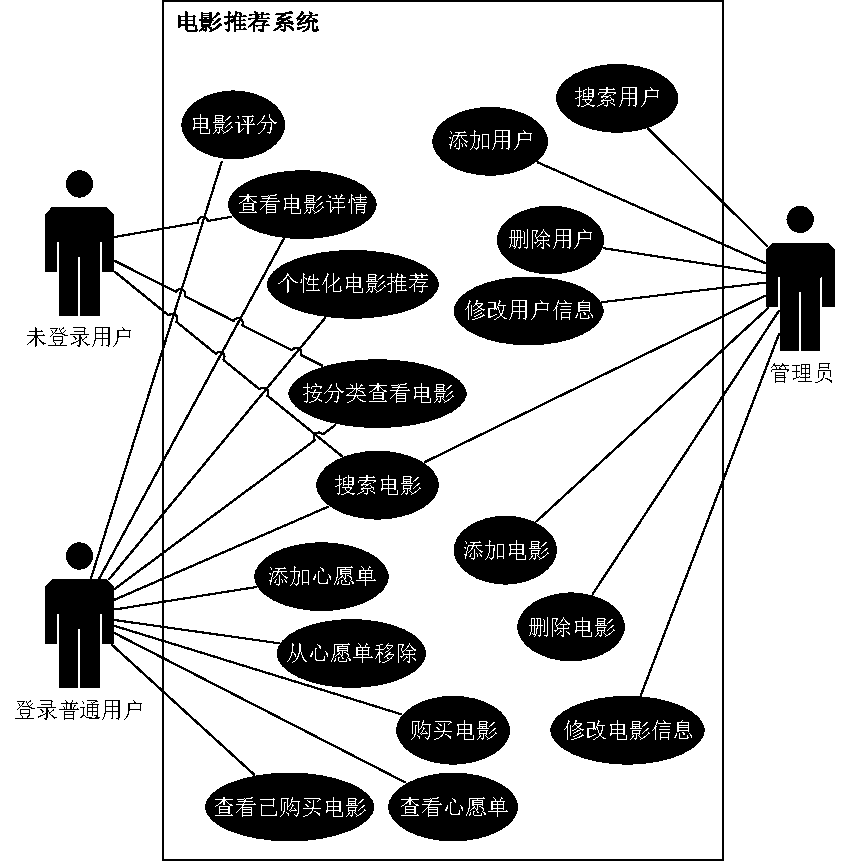
\includegraphics{figures/use-case.pdf}
	\bicaption{系统功能用例图}{Use case diagram for the system }\label{fig:use-case}
\end{figure}
本系统用户角色分为未登录用户、普通用户与管理员用户,其用例说明如图\ref{fig:use-case}。
\subsection{系统导航}
本系统使用浮动侧边栏作为导航方式,如图\ref{fig:admin-navigation}。点击侧导航栏右下角的固定的按钮可以将浮动侧边栏设为固定,再次点击后将取消固定。
\begin{figure}
	\fbox{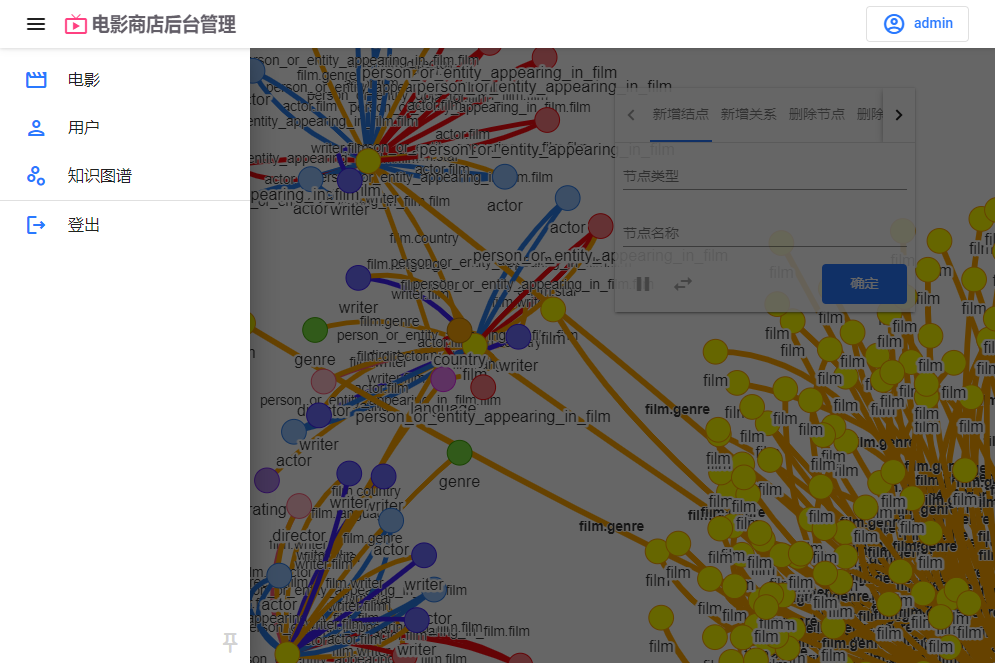
\includegraphics[width=.94\textwidth]{figures/admin-navigation.png}}
	\bicaption{系统侧导航栏(管理员)}{Side navigation panel of the system (for administrators)}\label{fig:admin-navigation}
\end{figure}

\subsection{未登录用户}
未登录用户能进行以下操作:

\noindent (1)接收随机的电影推荐

未登录用户首页随机显示50部电影,如图\ref{fig:anonymous-index}。
\begin{figure}
	\fbox{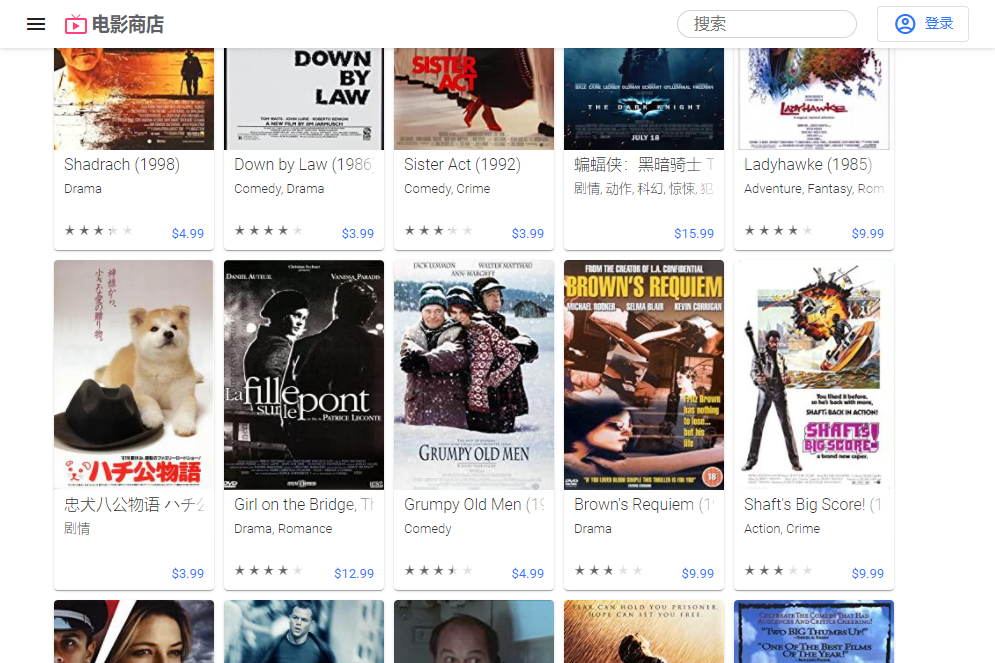
\includegraphics[width=.94\textwidth]{figures/anonymous-index.png}}
	\bicaption{未登录用户首页}{Index page for anonymous users }\label{fig:anonymous-index}
\end{figure}

\noindent (2)按分类查看电影

未登录用户可以根据电影的分类来查看电影,如图\ref{fig:anonymous-category}。
\begin{figure}
	\fbox{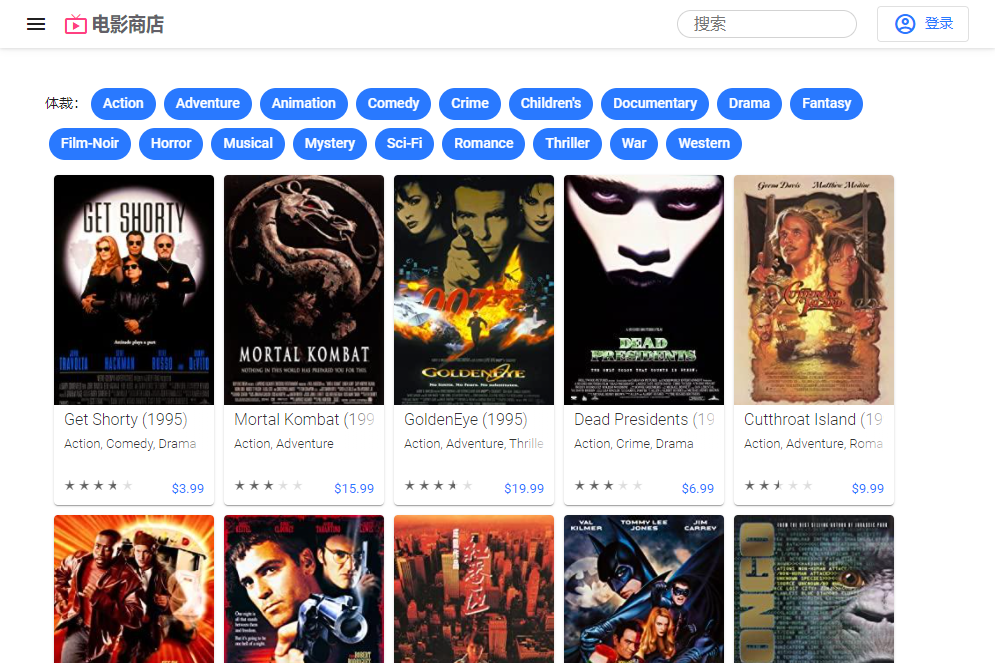
\includegraphics[width=.94\textwidth]{figures/anonymous-category.png}}
	\bicaption{未登录用户分类页面}{Category page for anonymous users }\label{fig:anonymous-category}
\end{figure}

\noindent (3)查看电影详情

未登录用户可以查看电影详情,如图\ref{fig:anonymous-details}。点击页面上的“添加至心愿单”和“购买”会跳转至登录界面。
\begin{figure}
	\fbox{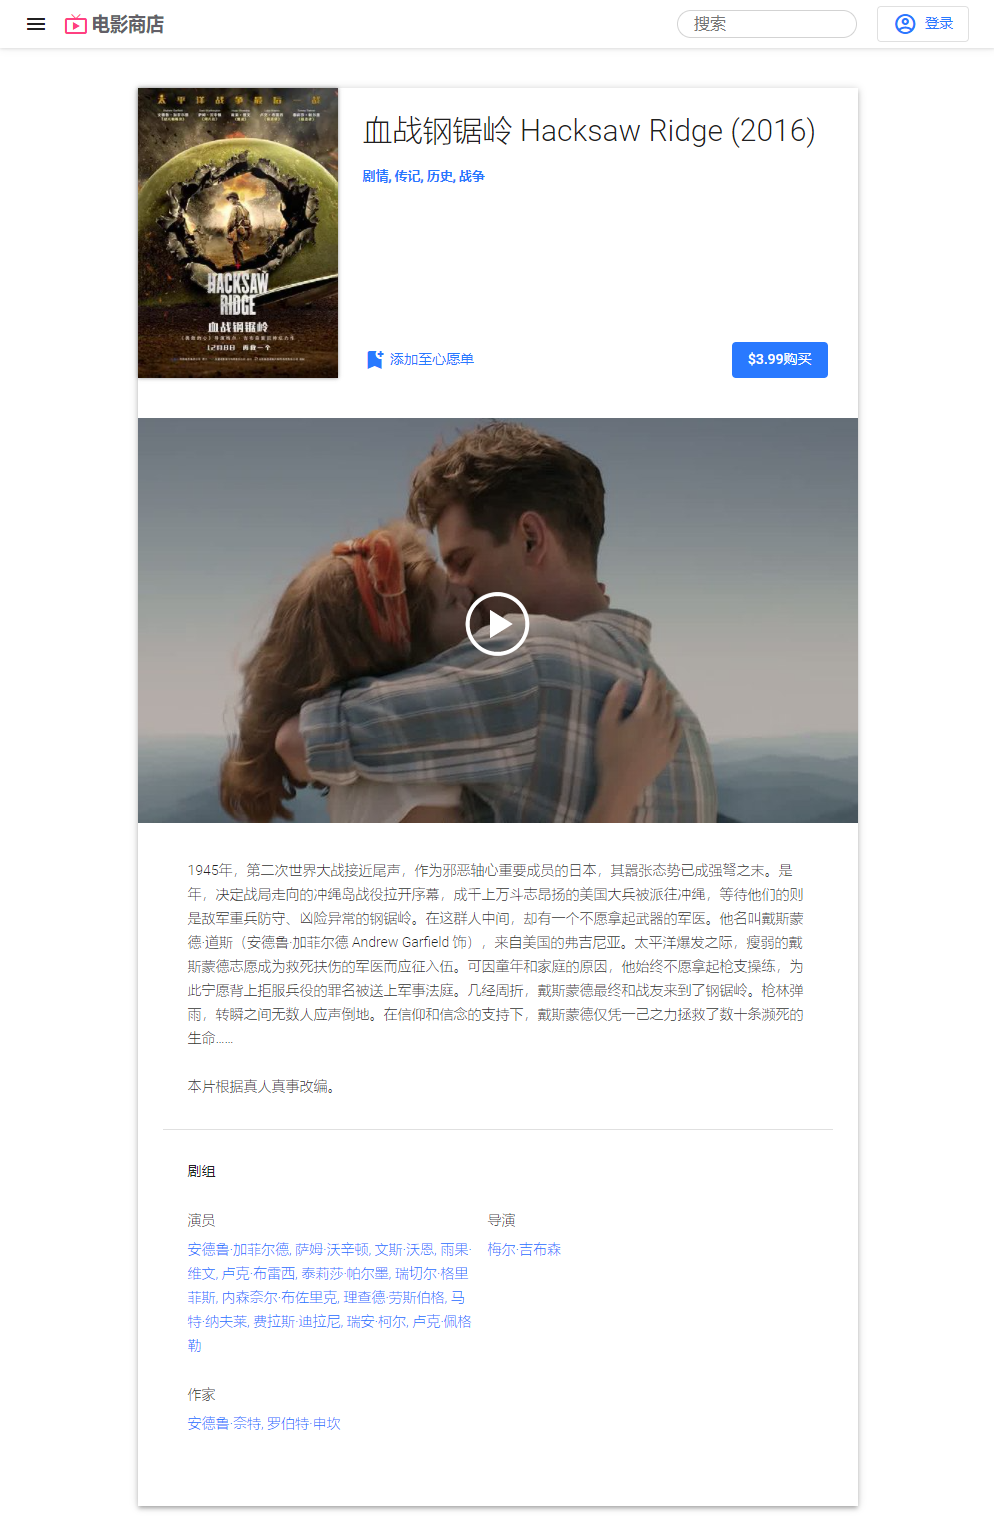
\includegraphics[height=.7\textheight]{figures/anonymous-details.png}}
	\bicaption{未登录用户电影详情页面}{Movie details page for anonymous users }\label{fig:anonymous-details}
\end{figure}

\noindent (4)搜索电影

未登录用户可以使用应用栏右侧的搜索框搜索电影,如图\ref{fig:anonymous-search}。本系统支持模糊搜索,与此同时,随着用户搜索内容的不断输入,系统会在搜索框下方显示候选的匹配词条,方便用户直接点击查看,此外,用户也能通过回车跳转至完整的搜索结果页面。
\begin{figure}
	\fbox{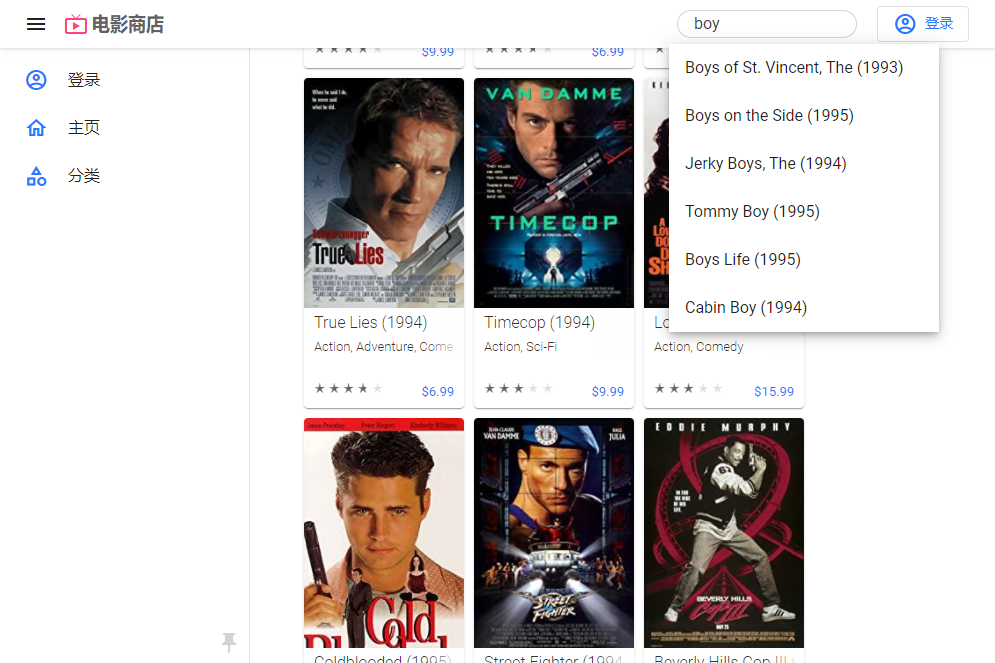
\includegraphics[width=.94\textwidth]{figures/anonymous-search.png}}
	\bicaption{未登录用户电影搜索界面(侧导航栏已固定)}{Movie search page for anonymous users (side navigation panel pinned)}\label{fig:anonymous-search}
\end{figure}
\subsection{注册与登录}
\noindent(1)注册

本系统对普通用户开放注册功能,并能提供用户名是否含不合法字符、是否与已注册用户名冲突、密码是否符合复杂度要求等的检测。

\noindent (2)登录

本系统提供登录功能,并能根据不同的登录错误类型相应地作出响应。
\subsection{普通用户}
普通用户具备未登录用户的所有功能。此外,还具备以下功能:

\noindent (1)添加心愿单

已登录用户能在电影详情页面添加电影至心愿单。

\noindent (2)购买

已登录用户能在电影详情页面购买电影。

\noindent (3)评分

已登录用户能在电影详情页面给电影评分。电影评分功能位于电影详情页面,如图\ref{fig:general-details}所示。

\begin{figure}
	\fbox{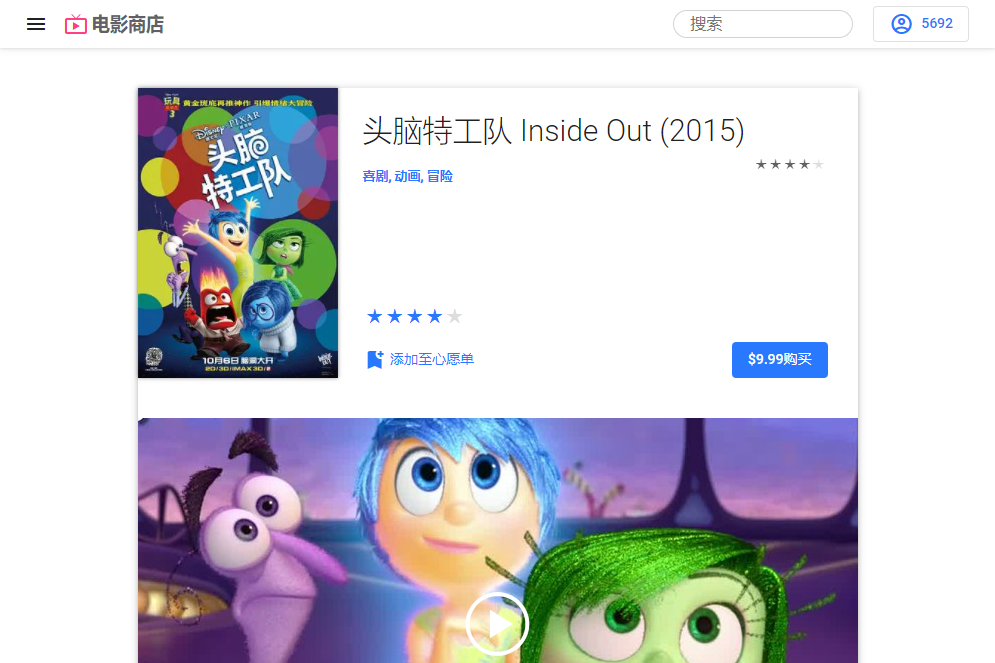
\includegraphics[width=.94\textwidth]{figures/general-details.png}}
	\bicaption{电影评分页面}{Rating page for movies}\label{fig:general-details}
\end{figure}

\noindent (4)查看已购买的电影

已登录用户能通过侧导航栏跳转至查看已购买的电影的页面。

\noindent (5)查看已添加心愿单的电影

已登录用户能通过侧导航栏跳转至查看已添加心愿单的电影的页面。
\subsection{管理员用户}
\noindent (1)管理电影信息

管理员能增加电影、删除电影与修改电影信息,如图\ref{fig:admin-movie}所示。
\begin{figure}
	\fbox{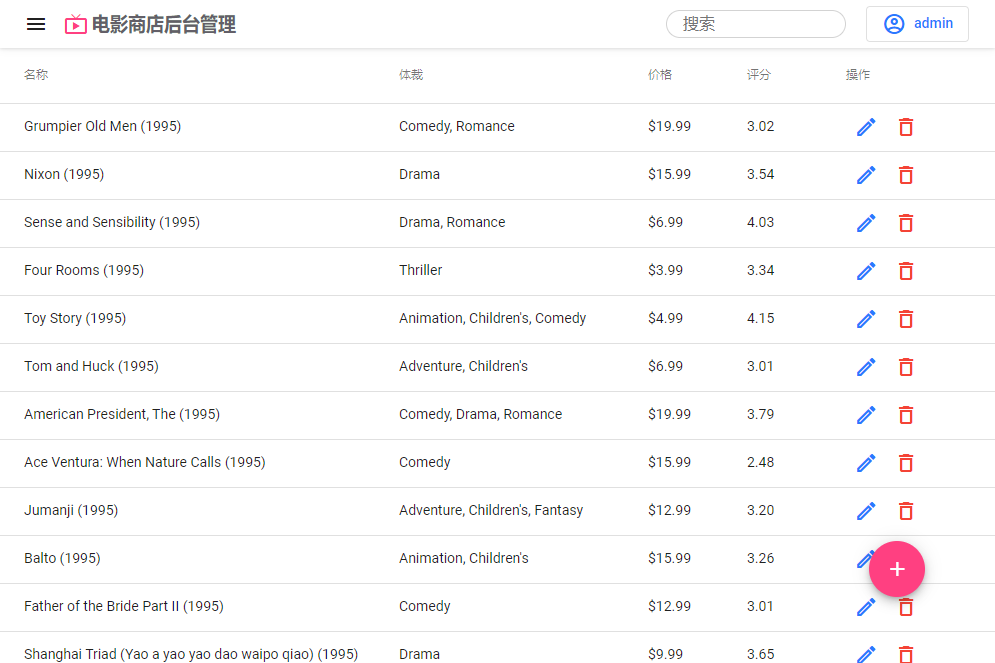
\includegraphics[width=.94\textwidth]{figures/admin-movie.png}}
	\bicaption{管理电影页面}{Movie administration page}\label{fig:admin-movie}
\end{figure}

\noindent (2)管理用户信息

管理员能增加用户、删除用户与修改用户密码。

\noindent (3)管理知识图谱

管理员能增加、删除、修改以及查找知识图谱中的结点与关系,如图\ref{fig:admin-knowledge-graph}所示。该界面中的结点及关系可以以动态的方式呈现,同时支持以填写选项的方式以及使用Cypher语句的方式来增加、删除、修改以及查找知识图谱中的结点与关系。当鼠标悬浮于某一节点或关系之上时,将显示有关这一节点或关系的有关信息。
\begin{figure}
	\fbox{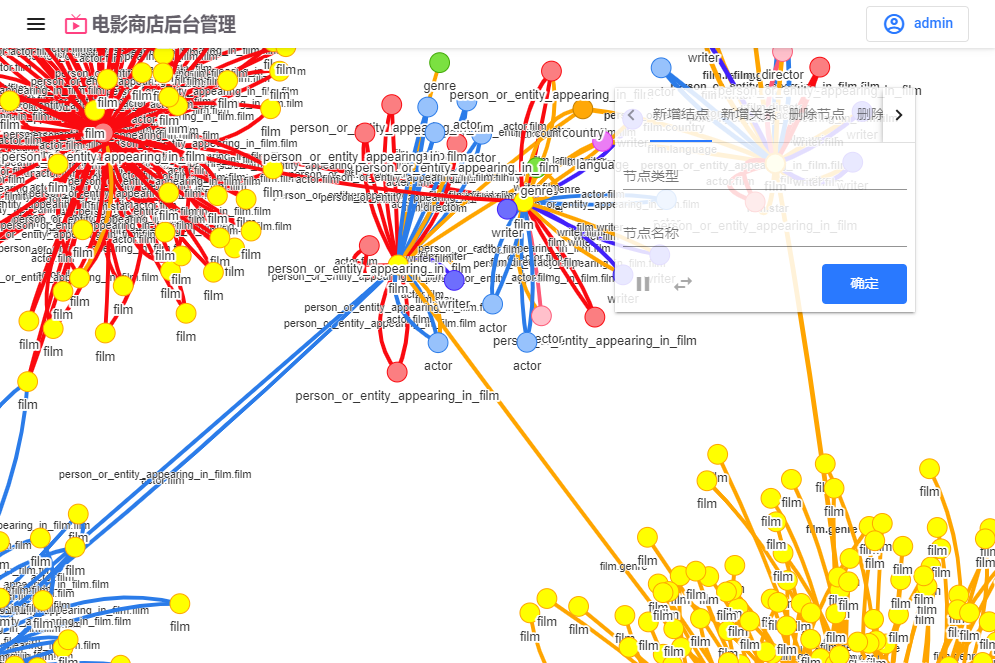
\includegraphics[width=.94\textwidth]{figures/admin-knowledge-graph.png}}
	\bicaption{管理知识图谱页面}{Knowledge graph administration page}\label{fig:admin-knowledge-graph}
\end{figure}
\section{电影推荐流程}
本系统的推荐流程分为离线推荐与实时推荐,如图\ref{fig:recommendation-procedure}所示。

\begin{figure}
	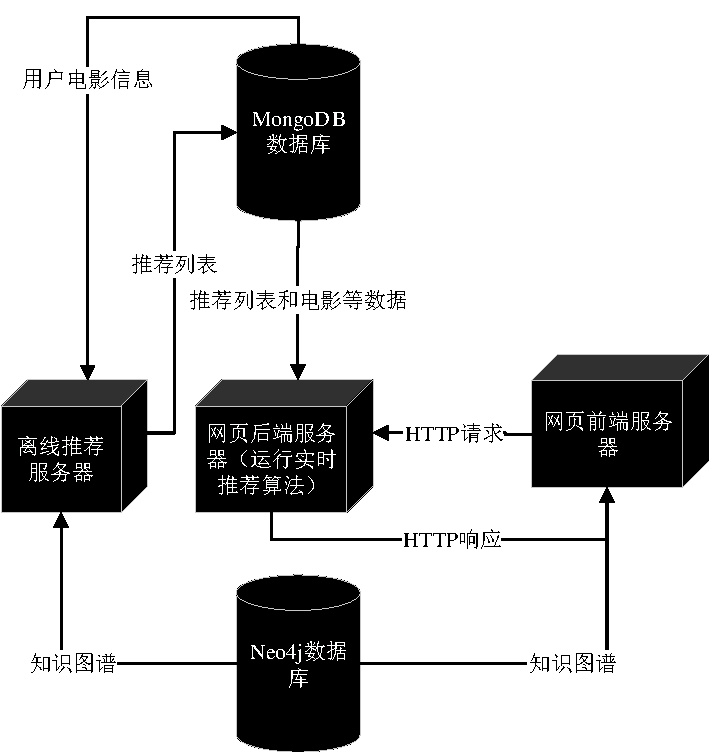
\includegraphics{figures/recommendation-procedure.pdf}
	\bicaption{电影推荐流程}{Movie recommendation procedure}\label{fig:recommendation-procedure}
\end{figure}

其中,离线推荐使用第\ref{ch:offline-recommendation}章所述的涟漪网络算法,此算法是基于文献\parencite{wang2018ripplenet}实现的。不同于文献\parencite{wang2018ripplenet}中仅使用用户评分计算用户偏好,本推荐系统在用户偏好的计算过程中还结合了用户收藏,这在一定程度上缓解了冷启动问题并改进了推荐性能。
此外,本推荐系统还结合了实时推荐机制作为补充,描述如下:

(1)离线推荐服务器定期运行涟漪网络算法。离线推荐服务器从MongoDB数据库服务器获取用户信息与电影评分、电影是否加入心愿单等数据以及从Neo4j数据库服务器获取知识图谱数据信息。然后执行涟漪网络算法。最后离线推荐服务器将计算得到的各用户推荐列表存入MongoDB数据库中,等待用户访问时将该结果推荐给用户。

(2)当用户访问时,网页后端服务器查询推荐列表中的电影数据是否达到阀值,如果推荐列表中的数量过少,则根据用户交互随机将同体裁电影加入推荐列表的末端作为补充并最终显示给用户。

上述步骤中,(1)中的离线推荐准确度高,但算法运算时间长,无法做到即时响应用户请求。(2)中的实时推荐方法准确度低,但算法运算快,可以做到实时响应请求并即时发出响应。两者相互补充组成了本系统的电影推荐算法。
\section{系统安全性}
本系统对已登录普通用户与管理员在前后端交互过程中使用JSON网络令牌(JSON Web Token, JWT)实现授权与认证(Authorization and Authentication),以此保证系统的安全性,本系统的总体安全性设计如图\ref{fig:jwt}所示。

\begin{figure}
	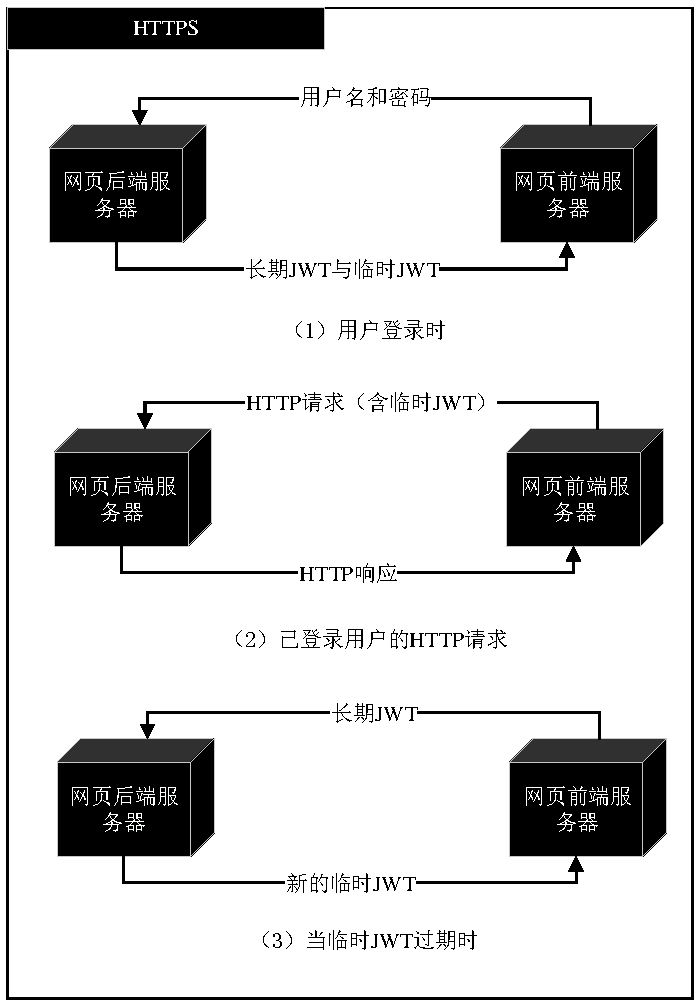
\includegraphics{figures/jwt.pdf}
	\bicaption{系统总体安全性设计}{Overall security design for the system}\label{fig:jwt}
\end{figure}

在用户登录时,Flask后端网页服务器会生成一个长期JSON网络令牌和一个临时JSON网络令牌,令牌中存储有用户id以及过期时间,并且该令牌使用非对称加密算法加密,其中含有由Flask后端网页服务器颁发的签名信息,这确保了JSON网络令牌不会被伪造。

前端网页服务器在接收到令牌后会将令牌存储在浏览器的localStorage中,并在每一个接下来的请求头中附上该令牌,而后端服务器只有在该令牌有效(指确实为后端网页服务器颁发且该另令牌尚未过期)的情况下才会继续执行有关请求。与此同时,若该请求是用户内容相关的,则后端服务器还会检测令牌中的id是否与请求中使用的id相同。若不满足以上任意一项,则后端网页服务器返回未授权错误。

其中,若后端网页服务器发现令牌过期,则会将该信息发送给前端网页服务器,前端网页服务器将会将长期令牌发送给后端服务器以刷新(renew)临时令牌。

此外,本系统还使用了哈希算法对密码进行哈希处理,数据库中的密码全部为哈希处理后的密码。同时,用户登录过程是后端网页服务器使用原密码与哈希处理后的密码进行比较,而没有开放哈希处理后的密码与哈希处理后的密码进行比较的接口,这保障了本系统的安全性。这在同时令网站仅允许HTTPS(HTTPS-only)网络连接的情况下可以充分保证本系统的安全性。

需要指出的是,虽然本系统在用户登录与注册时密码在前端没有进行哈希处理,但是本系统在部署时使用HTTPS-only的连接,在这种情况下,所有的数据传输都处于加密状态,避免了中间人攻击的可能,因此明文传输密码而不使用哈希处理是安全的,在实际使用的过程中可行。而本系统的后端网页服务器对前端网页服务器传入的明文密码进行哈希处理的目的是避免数据库中存入明文的密码。如果数据库中存入明文的密码,则当数据库中用户密码泄露时攻击者可以轻易使用泄露的密码登录本系统。而如上所述,本系统后端只开放了接收明文密码的接口,即只将数据库中哈希处理后的密码与用户请求中的明文密码进行对比,即使攻击者获取了用户哈希后的密码,要计算其对应的明文密码也是困难的,甚至在明文密码足够复杂的情况下是不可能的。因此,以上措施保证了本系统的安全性。
\chapter{研究结论和展望}
\section{工作总结}
随着互联网的发展,用户可选择的电影数量不断增加,为了让用户快速找到感兴趣的电影,各种推荐算法应运而生。这些算法存在推荐准确性较低、数据稀缺性以及冷启动问题。本文针对此现状,以电影推荐为研究对象,使用知识图谱作为辅助信息,利用涟漪网络算法实现了电影推荐系统。具体地说,主要的研究工作如下:

(1)使用基于Scrapy框架的爬虫从IMDb和豆瓣网上爬取了3684条电影数据。其中,从IMDb爬取了3494条电影数据,从豆瓣网爬取了190条电影数据(由于豆瓣网限制了每IP访问量故爬取的数据较少)。这些电影数据包括电影封面图片、电影情节介绍、电影预告片图片、电影演员列表、导演以及剧本作家等信息。

(2)根据文献\parencite{wang2018ripplenet}实现了基于知识图谱的涟漪网络推荐算法,通过使用“MovieLens 1M Dataset”数据集以及从IMDb和豆瓣网上爬取的电影数据,实现了基于用户心愿单和用户评分并以知识图谱为辅助信息的推荐算法。不同于文献\parencite{wang2018ripplenet}中仅使用用户评分计算用户偏好,本文在用户偏好的计算过程中还结合了用户收藏,这在一定程度上缓解了冷启动问题并改进了推荐性能。并对实现的推荐算法进行了实验,计算了其AUC和准确度两个关键的性能指标,将该指标与DKN\cite{wang2018dkn}、CKE\cite{zhang2016collaborative}、PER\cite{yu2014personalized}、SHINE\cite{wang2018shine}、LibFM\cite{rendle2012factorization}以及Wide\&Deep\cite{cheng2016wide}算法的进行了对比。并以此发现,涟漪网络算法的性能最优。

(3)基于涟漪网络算法实现了基于知识图谱的电影推荐系统。该系统为未登录用户提供按分类查看电影、查看电影详情的功能;为普通用户提供电影推荐、按分类查看电影、查看电影详情、电影评分、将电影加入心愿单以及购买电影功能;为管理员提供增加、删除、修改、查找电影及用户的功能。同时使用JSON网络令牌、HTTPS以及哈希化密码等手段保障系统的安全性。
\section{工作展望}
为了给用户提供准确的推荐电影,需要不断优化并改进推荐过程。推荐系统的基础是用户历史偏好集、知识图谱信息以及推荐算法本身。因此有效地记录用户历史偏好集,完善知识图谱信息并改进推荐算法本身是提高推荐结果的重要因素。本文虽然对基于知识图谱的推荐算法有了一定的研究,并且将其应用于电影推荐系统中,但是由于时间和能力所限,该系统仍存在着不足的地方,主要体现在以下两个方面:

\noindent (1)需要完善知识图谱的信息

知识图谱是本文使用的涟漪网络算法的基础,但本文所使用的知识图谱的信息还不够完善,因此在一定程度上影响了涟漪网络算法的性能。

\noindent (2)涟漪网络算法有待进一步改进

尽管涟漪网络算法相比于传统的推荐算法在准确度上有所提升,但涟漪网络算法目前仅适用于离线推荐,而无法用于实时推荐,这使它的适用场景受到了限制。未来可考虑改造该算法,使其能满足实时推荐的需求。

对于以上提及的问题,未来还需要更深入地学习有关知识图谱、推荐算法、深度学习的有关知识,对系统进行改进,从而使其更完善。
	\backmatter
    \printbibliography
	\chapter{致谢}
论文的撰写工作已经接近尾声,在本文的撰写过程中我要特别感谢李冬梅老师的指导。在毕业论文完成期间,李冬梅老师多次对我的毕业论文提出意见与建议。同时,她多次询问论文的撰写进度,更是体现了她对学生无微不至的关怀。每每当我在论文编写中遇到艰深晦涩之处时,她都能不失时机而恰到好处地给予我最有用的提示与建议,使我的毕业论文得以顺利完成。

其次,我要感谢我本科期间曾经为我上课的所有老师。比如,由我的概率论老师为我打下的数学基础才使我得以用最大后验概率估计法完成嵌入表示的学习算法,蓝海洋老师任教的网站设计课程是我完成电影推荐系统的基石。总之,我要感谢大学四年来所有老师孜孜不倦的谆谆教诲与夜以继日的无私奉献。

接着,我还要感谢我的同学,是他们思维的火花激起了论文写作中的灵感。与他们的交流使我受益匪浅。

最后,我还要感谢我的父母,他们一直以来对我生活上与学习上的鼓励与引导是我得益完成论文的关键要素。

感谢所有在论文撰写工作中为我提供过帮助的人。
\end{document}
